\documentclass{article}
\usepackage[nonatbib]{neurips_data_2021}
\usepackage[sort&compress,numbers]{natbib}
\usepackage[utf8]{inputenc}
\usepackage[urlcolor=blue,citecolor=blue,breaklinks,colorlinks]{hyperref}
\usepackage{url}
\usepackage[capitalize]{cleveref}
\usepackage{graphicx}
\usepackage{subcaption}
\usepackage{microtype,xcolor,booktabs}
\newcommand{\tbo}[1]{\textcolor{teal}{/* TBo: #1 */}}
\title{The CPD Data Set: Personnel, Use of Force, and Complaints in the Chicago Police Department}

\author{%
  Thibaut Horel\\
  LIDS, MIT \\
  \texttt{thibauth@mit.edu } 
  \And
  Lorenzo Masoero\\
  CSAIL, MIT \\
  \texttt{lom@mit.edu } 
   \And
 Raj Agrawal\\
  ArbiLex\\
  \texttt{r.agrawal@csail.mit.edu } 
   \And
  Daria Roithmayr\\
  Gould School of Law \\
  University of Southern California  \\
  \texttt{droithmayr@law.usc.edu}
 \And 
 Trevor Campbell \\
  Department of Statistics \\
   University of British Columbia\\
  \texttt{trevor@stat.ubc.ca}
}

\begin{document}


\maketitle

\begin{abstract}
\looseness=-1\relax
The lack of accessibility to data on policing has severely limited researchers'
ability to conduct thorough quantitative analyses on police activity and
behavior, particularly with regard to predicting and explaining police
violence. In the present work, we provide a new dataset that contains
information on the personnel, activities, use of force, and complaints in the
Chicago Police Department (CPD). The raw data, obtained from the CPD via a
series of requests under the Freedom of Information Act (FOIA), consists of 35
unlinked, inconsistent, and undocumented spreadsheets. Our paper provides a
cleaned, linked, and documented version of this data that can be reproducibly
generated via open source code. We provide a detailed description of the
dataset contents, the procedures for cleaning the data, and summary statistics.
The data have a rich variety of uses, such as prediction (e.g., predicting
misconduct from officer traits, experience, and assigned units), network
analysis (e.g., detecting communities within the social network of officers
co-listed on complaints), spatiotemporal data analysis (e.g., investigating
patterns of officer shooting events), causal inference (e.g., tracking the
effects of new disciplinary practices, new training techniques, and new
oversight on complaints and use of force), and much more. Access to this
dataset will enable the machine learning community to meaningfully engage with
the problem of police violence.
\end{abstract}

\textbf{Repository: \url{https://github.com/chicago-police-violence/data}}\\
\textbf{Instructions:} run \texttt{make} in the repository's root directory.
See \texttt{README.md} for detailed instructions.\\
\textbf{Data Set:} may be found in the \texttt{final/} directory after running \texttt{make} and is downloadable as a ZIP file at \url{https://github.com/chicago-police-violence/data/releases/download/v0.1-pre/cpd-dataset-v0.1-pre.zip}.

\section{Introduction}

There has been some ML work done on individual correlates that are associated
with (and potentially predictive of) police misconduct. Scholars have looked at
the association between misconduct and an individual officer's race, gender,
years on the force, prior instances of misconduct, stages of officer career,
assigned unit. But research suggests that violence emerges not just at the
individual level but also at the population level from the interaction of
individuals in groups—think of gangs. 

 
We offer a dataset that allows ML to investigate the influence of police social
networks on police misconduct. The dataset allows ML to explore features of
police social networks that might be associated with and potentially predictive
of adverse police encounters with civilians or other misconduct. These network
correlates can include the architecture and structures of social networks in
departments and smaller subunits within a department—for example, the number of
connections each officer has, the strength of those connections, the bridge
positions that some officers have across subunits. More innovatively, ML can be
used in the way it is often used to study disease dynamics: ML can find the
patterns of behavior (clustering, outbreaks, spreading, geographic hotspots) on
a network that might be associated with violence. 

 
We show how to use complaint datasets from a police department in a major city
to investigate the influence of social networks on police misconduct and
violence. 


The original data was obtained following a series of requests covered by the
Freedom of Information Act (FOIA) to the Chicago Police Department (CPD) and
the Civilian Office of Police Accountability (COPA). The information which was
requested pertained to CPD's personnel and its activities.

\textbf{TODO:} ideally say a bit more about the history of these FOIA requests.
Apparently they were initiated by individual journalists and lawyers and were
later coordinated by the Invisible Institute which ultimately became the
central location were (almost) all the data is currently available.

\begin{table}[h]
	\begin{center}
\begin{tabular}{@{}llll@{}}
	\toprule
	request \#&received&requested&description\\
\midrule
	\texttt{P0-58155}&2017-04-17& &Officer roster\\
	\texttt{P4-41436}&2018-03-21& &Officer roster\\
		\texttt{P0-52262}&2016-12-04&2016-09-19&Unit assignment\\
		\texttt{16-1105}&2016-03-11&2016-02-10&Unit assignment\\
	\texttt{P0-46957}&2016-06-29&2016-04-22&Complaints (CPD)\\
	\texttt{18-060-425}&2018-08-28&2018-08-20&Complaints (COPA)\\
	\texttt{P0-46360}& & &Tactical Response Reports\\
\bottomrule
\end{tabular}
\caption{Summary of the FOIA requests to the CPD and COPA contained in our repository.}
\label{table:summary}
\end{center}
\end{table}

Each FOIA request is identified by a request number, \cref{table:summary} gives
an overview of all the requests made to the CPD and COPA that are present in
our repository. This information is also available in the file
\texttt{dataset.csv} in the root folder of the repository. The original
data—that is the files received after each FOIA request—are present in the
\texttt{raw/} folder of the repository, with one subfolder for each request,
identified by the request number. When available, each subfolder also contains
the formal request letter as well as the reply letter from the CPD or COPA,
which are useful in understanding what data was included in each dataset.
Some additional comments about the data:
\begin{itemize}
	\item \emph{Officer roster:} lists all officers (past or present) employed
		by the CPD along with attributes such as year of birth, age, race,
		gender, appointment date, resignation date, etc.
	\item \emph{Unit assignment:} the CPD is organized into (500 or so?) units.
		Each officer can be assigned to one or multiple units and these
		assignments can change over time. The unit assignment datasets contain
		one record for each officer and each unit they were assigned to, with
		the start date and end date of this assignment.
	\item \emph{Complaints:} formal complaints filed by citizens against police
		officers. Complaints are identified by a complaint number, and there is
		one record for each complaint and each officer listed on the complaint,
		indicating the allegation made against them, result of the
		investigation of the allegation (with possible sanction), etc.
	\item \emph{Tactical Response Reports:} these are forms that officers are
		required to file after each incident for which the officer's response
		involved use of force.
\end{itemize}

Let us already mention an inherent difficulty in making use of this data, which
will be discussed in \cref{sec:linking}: there is no number/identifier which
uniquely identifies officers across datasets. Such an identifier probably
exists internally in the CPD, but was never included in the data released to
the public. One would be tempted to believe that the \emph{badge number} (also
sometimes referred to as \emph{star number} of an officer is such an
identifier, but unfortunately, it changes over the course of an officer's
career in the CPD, and a given badge number can be reassigned to different
officers when they are no longer in use.


\subsection{Related Work}

Police records datasets

This data was originally obtained by the Invisible Institute and has been publicly available for about 3 years here \url{https://github.com/invinst/chicago-police-data}
(limitations: not well organized or reproducible, problematic/incorrect linkage, missing unit information, units are not semantically grouped)

Gang violence data


\section{Related Work}\label{sec:related}

Existing public datasets on policing are extremely limited. All police
departments collect data on police personnel, activities, operations and
complaints, but few agencies disclose such data to the public \cite{Jackman21}.
A small but increasing number of departments are using the data to develop
machine learning approaches to “early intervention” warning systems that
predict adverse encounters between civilians and police. However, the datasets
used for these “early intervention systems” remain confidential, even when
scholars publish the results of their work on such systems \cite{Helsby18}.

In response to public pressure on the issue of police violence, a number of
public datasets on policing have recently emerged. These datasets, which are
generated by both private and public actors, are hard to reproduce and often
incomplete. For example, the Police Data Initiative (sponsored by a non-profit
on science in policing) is a collection of datasets from more than 130 state
and local law enforcement. These datasets often contain raw, uncleaned data,
and almost never include information about individual officer behavior
\cite{pdi}.  Stanford University’s Open Policing Initiative, which contains
data on traffic stops from around the country, does not include information
about identifiable individual officers \cite{sopp}.

The NYPD Misconduct Complaint Database, which has been compiled by the New York
Civil Liberties Union, includes complaint data made available by the New York
Police Dept.\ Civilian Complaint Review Board (a civilian oversight
organization.) This dataset includes information identifying officers by name
and is searchable as well, but the dataset includes only uncleaned data.
 
Current data collection efforts by government agencies can overcome some of
these limits, but can also face political and legal challenges. Owing to
political resistance by the Trump Administration, the Department of Justice
(DOJ) only began last year to collect data on arrest-related deaths through the
implementation of the ``Death in Custody Reporting Act'' of 2013. Under this
act, states are required to provide data regarding the death of any person
related to policing activity (detained, under arrest, in the process of being
arrested, etc.) But states often cannot compel local law enforcement to
disclose the data in the absence of state legislation. Likewise, the Federal
Bureau of Investigation (FBI) ``National Use-of-Force Data Collection'' program
is voluntary and not mandatory.

Policing scholars have compiled their own datasets. In a paper on the impact of
race and gender on policing, economist Bocar Ba and his research team generated
a publicly available dataset with information on individual officers in the
Chicago Police Department. This dataset linked officer demographic information
with their arrests, stops, assignment history, and data on the districts to
which the officers were assigned. Documentation for this dataset was
appropriate but sparse, making the reproduction of the dataset from scratch
somewhat challenging.

Other scholars have drawn on the same Invisible Institute data to create
a dataset similar to ours, but with far less documentation and focus on
reproducibility. In a paper on the impact of complaints on misconduct, Legal
scholars Rozema and Schanzenbach used the Invisible Institute raw data files to
link information on officer complaints with litigation settlements involving
the officers. However, neither the paper nor the publicly available dataset
provided any information about cleaning, processing or linking the data. 


\section{The CPD Data} \label{sec:data}
The original raw data released by the CPD, 
the code to generate the cleaned data, and the source code for this document 
are available at \url{https://github.com/chicago-police-violence/data}.
The data processing code is written in Python, and the documentation is written in \LaTeX.
\texttt{Make} is used to coordinate the various processing steps and easily reproduce them.
Refer to \url{README.md} in the repository for details regarding system requirements and 
how to generate the cleaned data.

\subsection{The raw data: origin, description, and challenges}
The first raw data files in this repository were obtained by J.~Kalven, an 
independent journalist, who filed Illinois Freedom of Information Act requests with 
the Chicago Police Department regarding complaints filed against officers. 
In Kalven v.~City of Chicago \cite{kalven2014}, an Illinois appellate court issued
a general ruling that documents bearing on allegations of
police abuse are public information. Following 
the decision, the non-profit
Invisible Institute began to collaborate with Kalven 
and the University of Chicago's Mandel Legal Aid
Clinic to follow up on earlier FOIA requests and to file new ones. The data
disclosed in response to these earlier and now ongoing FOIA requests were made available
online as part of the Citizens Police Data Project \cite{cpdp}.
These data form the basis of the cleaned and linked data set provided by the present work.

\begin{table}[h]
	\begin{center}
\begin{tabular}{@{}lllll@{}}
	\toprule
	request \#&received&requested&description\\
\midrule
	\texttt{P0-58155}&2017-04-17& &Officer roster\\
	\texttt{P4-41436}&2018-03-21& &Officer roster\\
	\texttt{P0-52262}&2016-12-04&2016-09-19&Unit assignments\\
	\texttt{16-1105}&2016-03-11&2016-02-10&Unit assignments\\
	\texttt{P0-46957}&2016-06-29&2016-04-22&Complaints (CPD)\\
	\texttt{18-060-425}&2018-08-28&2018-08-20&Complaints (COPA)\\
	\texttt{P0-46360}& & &Tactical Response Reports\\
	\texttt{P0-46987}&2016-05-13&2016-04-25&Unit names\\
	\texttt{P0-61715}& &2017-07-26&Awards\\
	\texttt{P5-06887}&2019-10-11&2019-07-19&Awards\\
	&2017-09-27&2017-09-13&Salary\\
\bottomrule
\end{tabular}
\caption{Summary of the FOIA requests contained in our repository (blanks are missing entries).}
\label{table:summary}
\end{center}
\end{table}

The raw data files are contained in the \url{raw/} folder of the
repository. Each subfolder corresponds to a FOIA request, which is
generally identified by a request number. \cref{table:summary} gives
an overview of all the requests that we include in
our repository; this meta-information is also included in the \url{raw/datasets.csv}
file in the repository. The subfolders contain the data provided by the city
in response to their corresponding FOIA requests, which typically comprises multiple
Excel spreadsheets. In addition, when available, the subfolders contain formal correspondence 
regarding the request, which often provides useful contextual information in understanding the data.  

In particular, the raw data files contained in the repository
provide the following information: {\color{red} todo: year ranges for each?}
\begin{description}
	\item[Officer roster:] a list of all officers (past and present) employed
		by the CPD along with attributes such as year of birth, age, race,
		gender, appointment date, resignation date, etc.
	\item[Unit assignments:] the CPD is organized into over 200 units.
		Each officer can be assigned to one or multiple units and these
		assignments can change over time. The unit assignment datasets contain
		one record for each officer and each unit they were assigned to, with
		the start date and end date of this assignment.
	\item[Complaints:] formal complaints against police officers, filed both by citizens
                and internally within the department. Complaints are identified by a complaint number. 
                There is one record for each complaint and each officer listed on the complaint,
		indicating the allegation made against them, result of the
		investigation of the allegation (with possible sanction), etc.
	\item[Tactical Response Reports:] these are forms that officers are
		required to file after each incident for which the officer's response
		involved use of force. Each record contains... {\color{red} thibaut fill in, similar to above for complaints}
        \item[Unit names:] the (human-readable) name of each (past and present) unit in the CPD. 
                Unit names also appear occasionally where unit numbers are listed in the other data files.
        \item[Awards:] a list of all awards requested for officers in the CPD, including 
                award tracking number, reference number, award type, request date, requester name,
                etc.
        \item[Salary:] a list of officers from 2002--2017 including their salary, position, and pay grade.
\end{description}

Challenges:
- time varying attributes: badge numbers (stars), unit numbers, job titles change over time. but 
more unusual things change too -- names (e.g.~marrying), appointment dates (e.g.~when db entries are corrected)
- systematic errors: unit history backwards, 
- multiple DBs: salary comes from different DB from the rest of it. names were entered differently, etc.
- ambiguous field meanings: salary has 2 different dates for apt, etc.
- dead entries: 
- inconsistent entries across different files: officers missing from history, roster, present in salary, etc
- idiosyncratic errors: 


\subsection{Initial Cleaning}

The files initially released by the CPD as a reply to the FOIA requests are for
the most part Excel spreadsheets, with inconsistent formatting and which can
thus be difficult to process programmatically. As an example, the reader is
invited to open the file
\texttt{p046957\_-\_report\_1.1\_-\_all\_complaints\_in\_time\_frame.xls}
available in the folder \texttt{raw/P0-46957/}. As can be seen, each record in
this file is spread over two rows of the spreadsheet, with the field names
repeated at the beginning of the second row for each record.

The goal of the cleaning step is thus to produce ``reasonable'' CSV files from
the original files, with the minimum requirement that each record be presented
on a single line after this step. The code for this cleaning step is contained
in the files \texttt{datasets.py}, \texttt{parse.py} and
\texttt{parse\_p046957.py} in the \texttt{src/} folder and the entire step can
be applied by running \texttt{make parse} in the root of the repository. This
creates the folder \texttt{parsed/} containing the clean CSV files.

As can be seen by inspecting the code, the decisions made at this stage are, we
believe, uncontroversial as they only consists of:
\begin{itemize}
	\item unifying field names across datasets, so that the same type of data
		is always identified in the saw way (for example, \texttt{Appointment
		Date}, \texttt{Appt Date}, \texttt{appointment\_date} are all mapped to
		\texttt{appointment\_date}.
	\item unifying field values across datasets. For example, the gender of an
		officer is indicated as a single letter \texttt{M} or \texttt{F} in
		some datasets or as \texttt{Male}, \texttt{Female} (based on the data
		release, it does not seem that the system used by the CPD has an option
		to represent non-binary officers).
	\item parsing values into the correct data type or format. For example,
		dates are formatted differently depending on the dataset, and we map
		everything to the ISO 8601 format.
\end{itemize}

Consequently, for someone planning to use the data in the present repository,
there is virtually no reason not to start at the minimum from the output of
this cleaning step. The subsequent steps required making more difficult and
debatable decisions, so depending on the application, researchers might want to
perform them differently, but in all cases, those alternative decisions can
branch off from the output of the cleaning step.

\subsection{Linking and Merging Datasets}\label{sec:linking}

\subsubsection{Officer matching}

As already alluded to, the main challenge at this step is that there is no
identifier uniquely identifying officers across records. In other words, there
is no foolproof way to know if two different records correspond to the same
officer, \emph{even within the same dataset} (for example the same officer
could appear with slightly different attributes on two different complaint
records).

We thus need to design a matching method striking a balance between
\begin{itemize}
	\item being loose enough to avoid type II error (false negatives). If the
		same officer appears with slightly different attributes across two
		records, we do not want our matching method to believe it is two
		different officers.
	\item being strict enough to avoid type I error (false positives). We do
		not want to merge two different officers into a single identity.
\end{itemize}

The difficulty in achieving this balance is that perhaps surprisingly
\emph{none of the attributes of a given police officer are guaranteed to be
stable over time}. Most notably, officers' names change over time, for example
to fix data entry errors or in case of legal name changes. However, we observed
two attributes, present in almost all original datasets and which seem
remarkably stable over the time: \emph{appointment date} and \emph{birthyear}.
These two attributes thus proved very valuable to disambiguate officers with
identical names.

In order to match officers across two datasets, we developed an \emph{iterative
pairwise matching procedure} that makes iterative passes over the datasets.
During each pass, a subset of the officer attributes present in both datasets
is selected as the matching criterion, and a pair of officers (one from each
dataset) is identified as a \emph{match} if (i) their attributes from the
chosen subset match, and (ii) if they are the only two officers matching on
these attributes. Once a pair is identified as a match, it is put aside, and
the next pass is performed on the remaining unmatched officers. After all the
passes are done the leftover officers are declared as different officers. By
constructing a hash table mapping a subset of attributes to the list of
officers sharing these attributes, each pass can be performed in linear time,
so the overall running time of the procedure is $O\big(P(N_1+N_2)\big)$ where
$P$ is the number of passes and $N_1, N_2$ are the number of officers in each
dataset.

To fully specify the matching procedure we thus need to specify which subset of
attributes is chosen as the matching criterion at each pass. For this, we go
from the stricter to the looser criterion: for the first pass, we choose
a subset \emph{all} the attributes which are present in two datasets, and then
start removing attributes one by one. For example, one can remove the
\emph{last name} attribute for the second pass to match a pair of officers
whose last names are different but match on all the remaining attributes, thus
identifying an officer whose last name changed between the releases of the two
datasets. The advantage of going from stricter to looser is two fold:
\begin{itemize}
	\item starting from the strictest set of attributes identifies the
		\emph{unambiguously matching pairs}, that is, the ones which are
		a clear match and which, thankfully, constitute the vast majority of
		officers (typically around 80-90\% of officers are matched during the
		first pass \textbf{TODO check}). Since the next passes will only be
		performed on the remaining unmatched officers, this removes a lot of
		potential ambiguities which could occur once the set of attributes is
		reduced.
	\item since the vast majority of officers is matched during the first pass,
		it becomes feasible during the subsequent passes to visually inspect all
		the matched pairs and assess whether the chosen set of attributes was
		too strict or too lose (\textbf{TODO:} explain how to activate
		debugging information in the code).
\end{itemize}

We note that there is still some amount of subjective judgment involved,
following a visual inspection of the second and subsequent passes, to decide
which sets attributes are ``acceptable'' (that is, for which the probability of
two persons sharing these attributes in a population of the size of the CPD is
extremely small). This is also how we decide that sufficiently many passes have
been performed: when it would seem likely to introduce a type I error by
matching any of the remaining officers. As a general rule of thumb we erred on
the side of favoring type II errors over type I errors. That is, we only
matched officers when it would seem extremely unlikely that they correspond to
two different individuals).

\textbf{TODO:} table of officer attributes in each dataset

\textbf{TODO:} explain the few subtleties where we don't use equality to match
attributes (for example when matching age and birthyear, where the age only
lets us identify the birthyear with an accuracy of 1 year). Or with stars,
where we test whether a star number is contained in the subset of known stars
for this officer.

With this procedure at hand we can thus link officers across datasets starting
from the most similar datasets first (for which we expect to have the least
amount of ambiguity). That is we first link \texttt{P0-58155} to
\texttt{P4-41436}, then \texttt{P0-52262} to \texttt{16-1105} and then the
remaining datasets \textbf{expand}

\textbf{TODO} give in appendix table summarizing which subset of attributes are
used at each linking operation 

\subsubsection{Roster consolidation}

A byproduct of matching officers across datasets is that for each officer, we
now have as many “profiles” as the number of datasets in which they appear,
where by \emph{profile} we mean a collection of attributes. Note that each
profile can contain a different subset of attributes (since not all attributes
are present in each dataset) and that a given attribute might take a different
value in different profiles of the same officer (since the iterative matching
procedure is not restricted to performing strict matching).

We are thus faced with the task of “consolidating” the different profiles of
a given officer into a single profile. Of course, if an attribute is present in
a single profile, and absent from the others, this is the value we keep in the
consolidated profile. But if an attribute appears with different values across
different profiles, we choose the value coming from the profile corresponding
to the \emph{most recent data release}.

\subsubsection{Unit assignment history} TODO.


\subsection{Unit identification and binning}


% !TEX root = ../main.tex

\section{Exploratory Analysis and Examples} \label{sec:analysis}

In this section, we provide examples and use-cases on the dataset. Code to
reproduce our examples is available online, in the \texttt{examples} folder.

\subsection{Visualizations}

\paragraph{Roster.}
%The file \texttt{roster.csv} contains information about $N=35{,}430$ CPD
%officers. For each officer --- identified by a Unique Identifier (``uid''),
%\texttt{roster.csv} provides, among other covariates, the officer's name,
%gender, race, birthyear, appointment and resignation dates. It is
%straightforward  to use the data to generate summary statistics, e.g., using
%appointment and resignation dates to understand the number of appointments,
%retirements as well as active officers over the years of  (\Cref{fig:history}).
%We report in \Cref{tab:stats} some 


\begin{figure}[t!] 
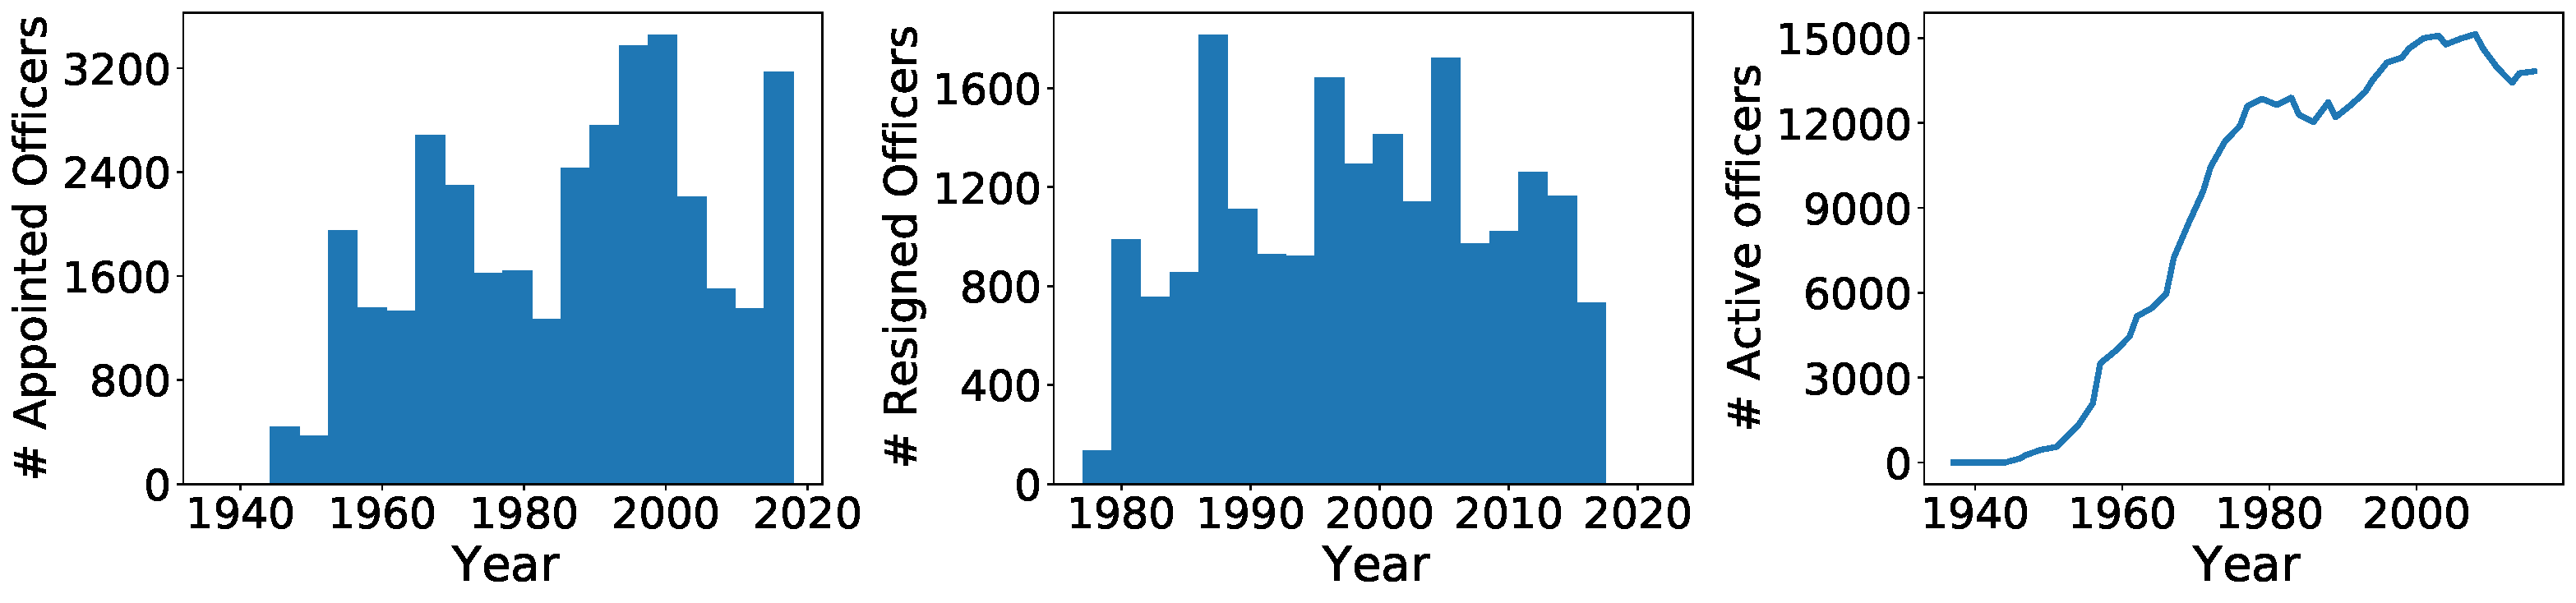
\includegraphics[width=\textwidth]{figs/history} 
\caption{Appointments (left), resignations (center), and the number of active
officers (right) appearing in the CPD roster database from the years 1940 to 2019.}
\label{fig:history}
\end{figure}

\begin{table}[t!]
\caption{Counts of officers (first row) and active officers (resignation date not before 2019-01-01, second row). 
Note that ``race'' and ``gender'' are per the CPD's coarse categorizations.} \label{tab:stats}
\begin{tabular}{l|c|c|c|c|c|c|c|c|c|}
\cline{2-3} \cline{5-10}
                                               & \multicolumn{2}{c|}{\textbf{Gender}} & \multicolumn{1}{l|}{} & \multicolumn{6}{c|}{\textbf{CPD Race Category}}                                                                                                                                                   \\ \cline{2-3} \cline{5-10} 
                                               & {\textbf{M}}   & {\textbf{F}}   &                       & {\textbf{White}} & {\textbf{Black}} & \multicolumn{1}{l|}{{\textbf{Hisp.}}} & {\textbf{Asian/P.I.}} & \multicolumn{1}{l|}{{\textbf{Indig.}}} & {\textbf{Bl. Hisp.}} \\ \cline{1-3} \cline{5-10} 
\multicolumn{1}{|c|}{\textbf{All}}    & 28316                 & 7122                  &                       & 21047                   & 8599                    & 4811                                         & 582                     & 67                                              & 9                           \\ \cline{1-3} \cline{5-10} 
\multicolumn{1}{|c|}{\textbf{Active}} & 11118                 & 4452                  &                       & 7241                    & 3895                    & 3596                                         & 467                     & 40                                              & 9                           \\ \cline{1-3} \cline{5-10} 
\end{tabular} 
\end{table}

\begin{figure}[h] 
	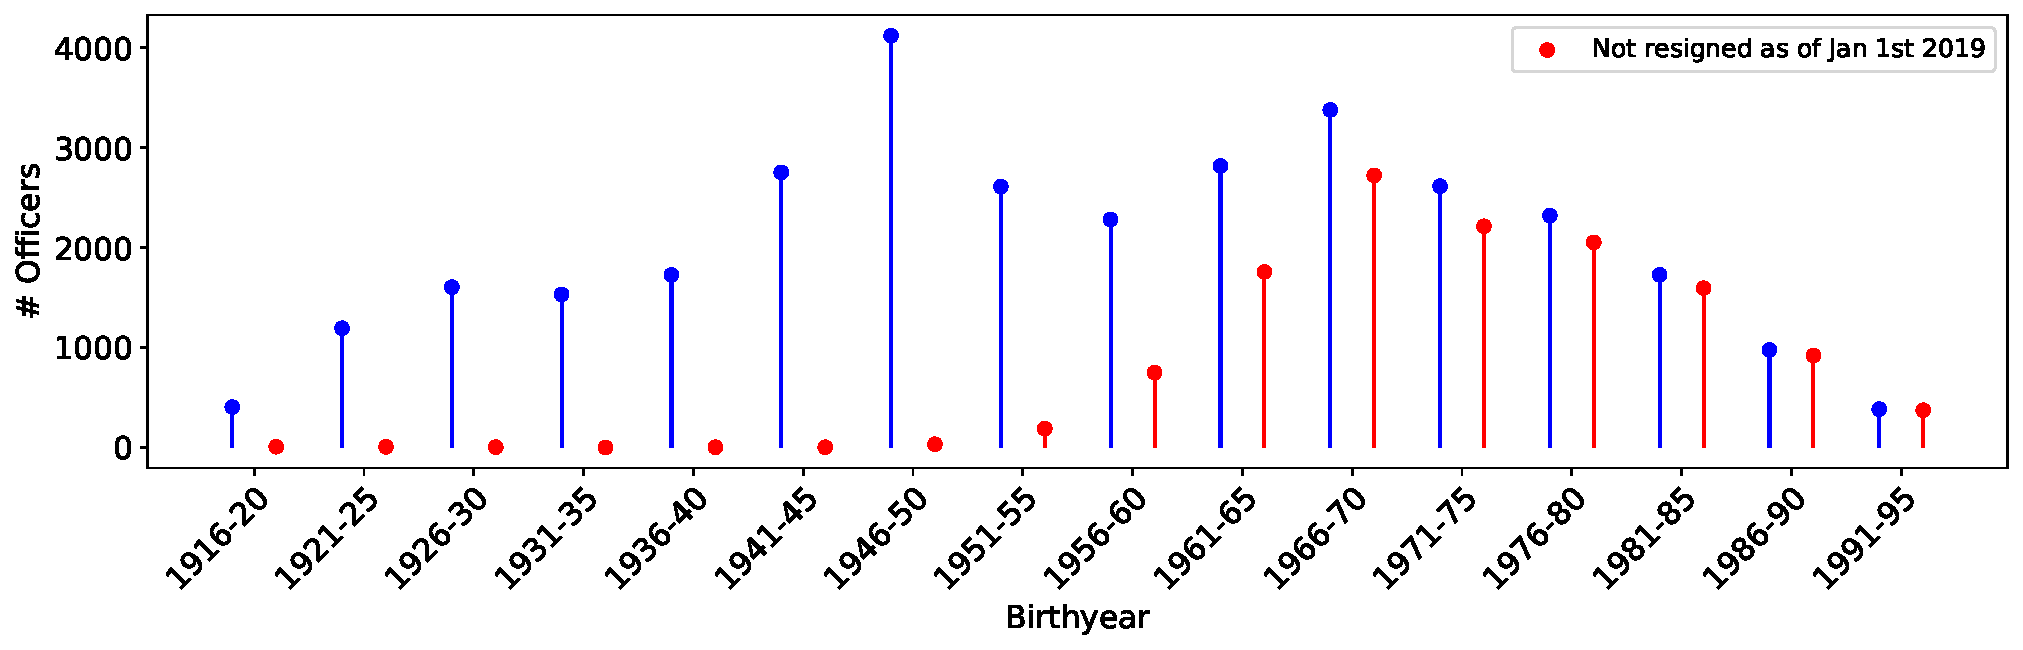
\includegraphics[width=\textwidth]{figs/history_by} 
	\caption{Historical data from the CPD. Birthyears for officers in the CPD dataset: blue dots count all officers, while red count only officers who are ``active'' as of January 1st, 2019.} \label{fig:history_by}
\end{figure}

We use the file \texttt{roster.csv} to obtain basic statistics about officers in the CPD dataset. The data contains informations about officers whose appointment dates back to 1936, all the way to 2018 (see \Cref{fig:history}). An important remark to be made is that the data becomes sparser, and less reliable in earlier years. For example, we report in the right subplot of \Cref{fig:history} the number of active officers (vertical axis) as a function of time (horizontal axis): we notice that this number increases sharply between 1940 and 1980. This should be interpreted as a consequence of the lack of data availability for those early years. We also report summary statistics on gender and the CPD race category in \Cref{tab:stats}, and information about officers' birthyears in \Cref{fig:history_by}.

\paragraph{Units.} 
\begin{figure}[h] 
	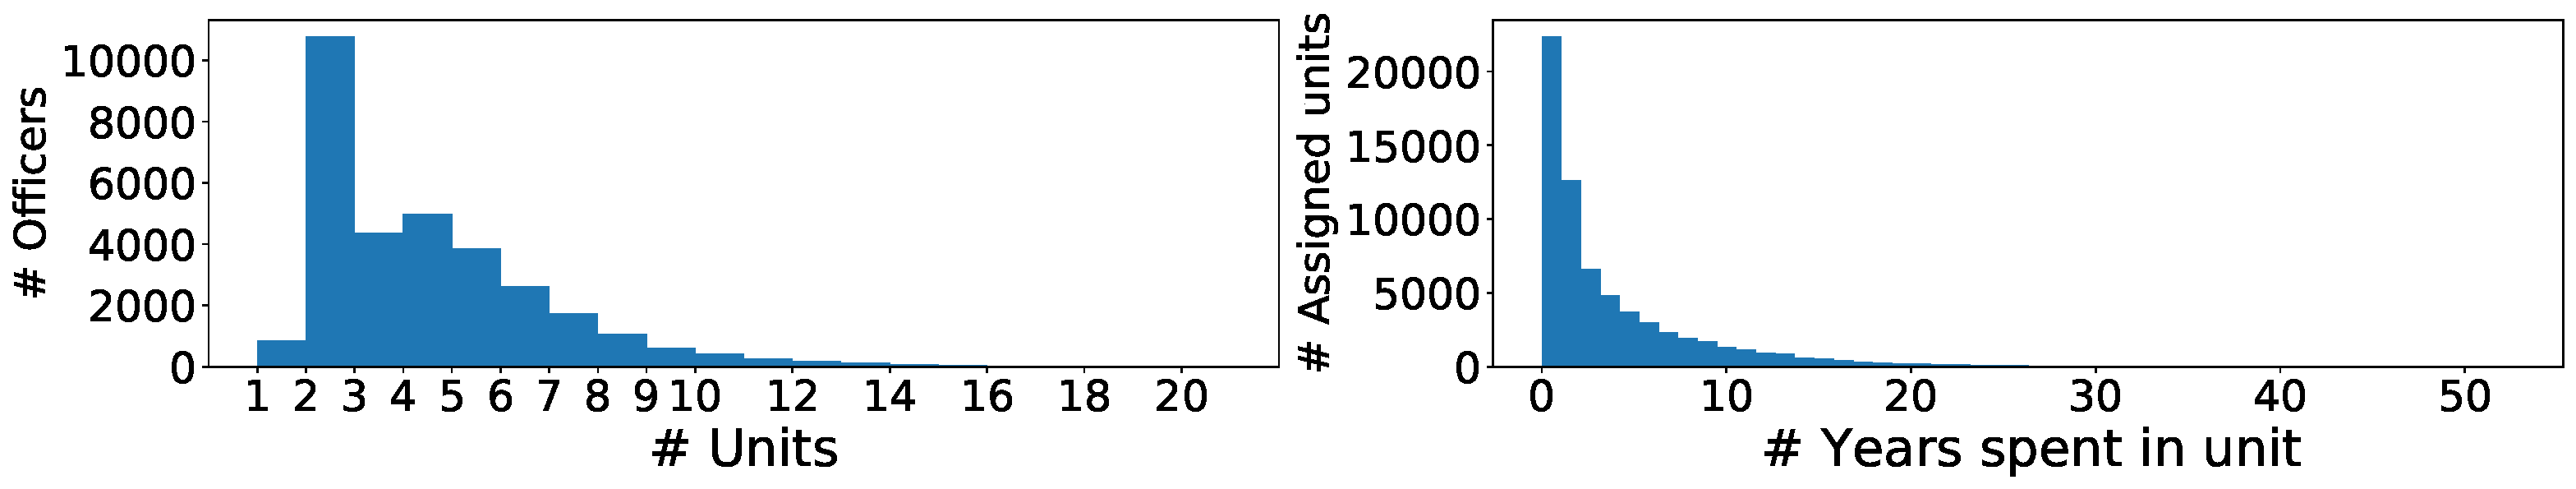
\includegraphics[width=\textwidth]{figs/units_officers} 
	\caption{Units assignments. Left: number of units assignments for officers in the CPD over the course of their career. Right: histogram for the number of years spent in each unit for ``completed'' units assignments only --- that is, assignments that had terminated at the time of data-collection.} \label{fig:units}
\end{figure}


We report summary statistics about the number of units an officer is assigned to, and the duration of such appointments in \Cref{fig:units}. The modal number of units appointments is 2: officers typically first joins the acadamy (unit 44), for one or two years, before moving on to a different, often terminal, unit. 
 
\paragraph{Complaints.} 
\begin{figure}[h] 
	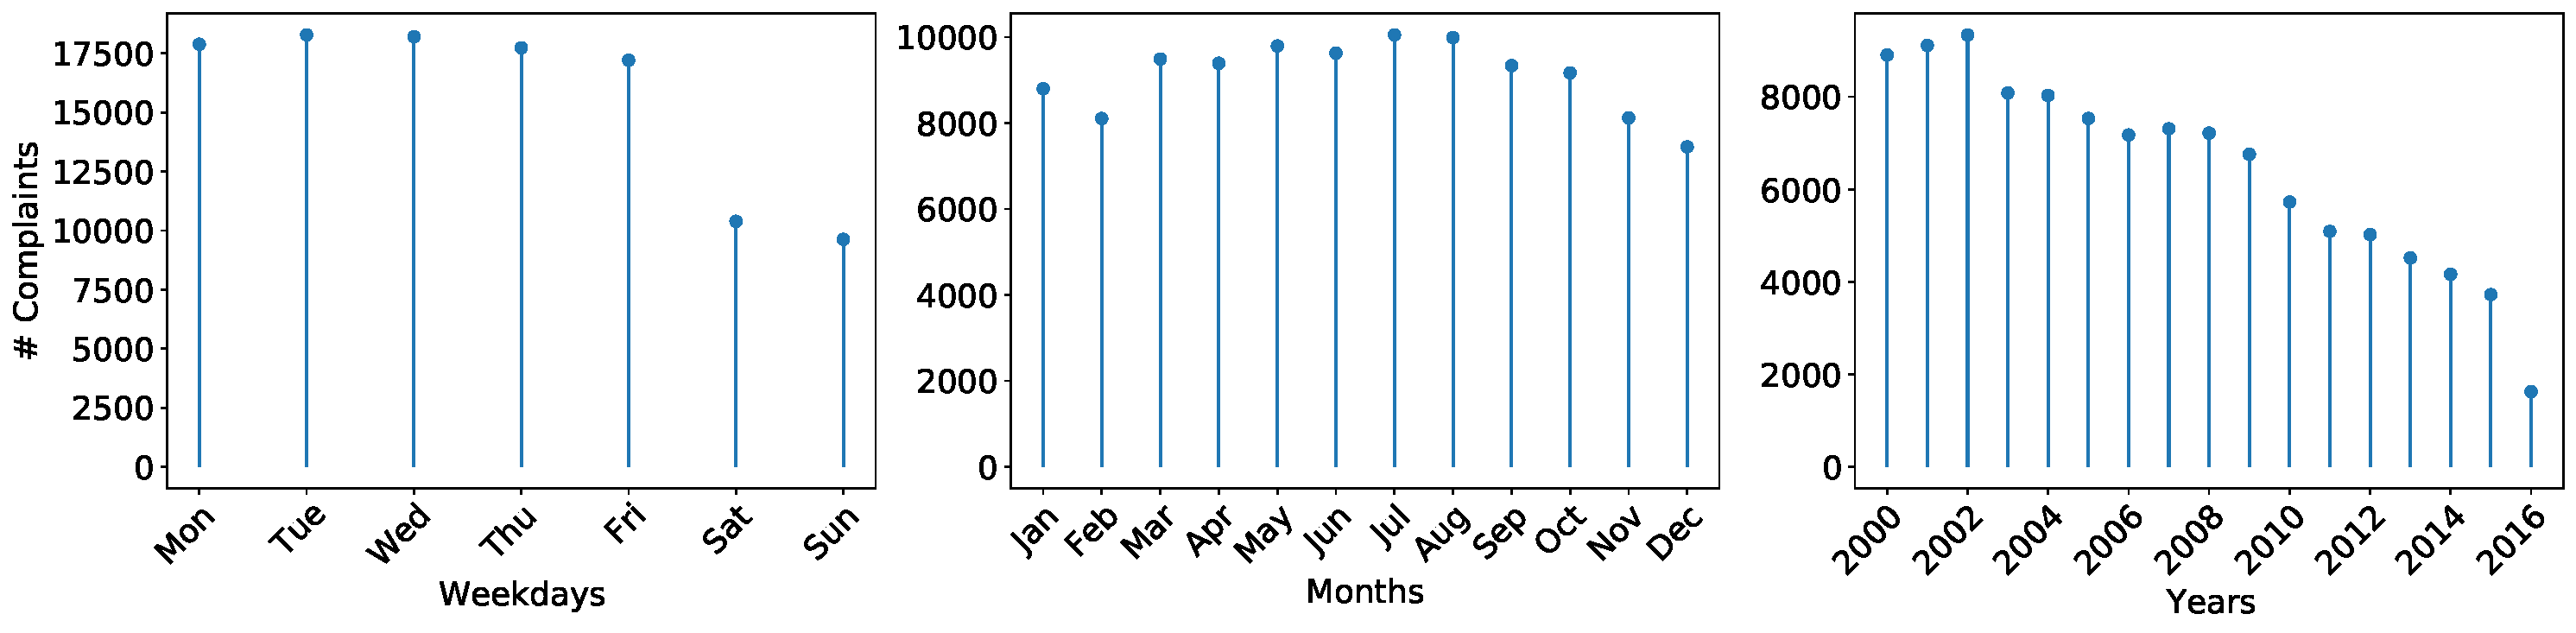
\includegraphics[width=\textwidth]{figs/complaints_times} 
	\caption{Temporal data for complaints.} \label{fig:complaints_times}
\end{figure}
\begin{figure}[h] 
	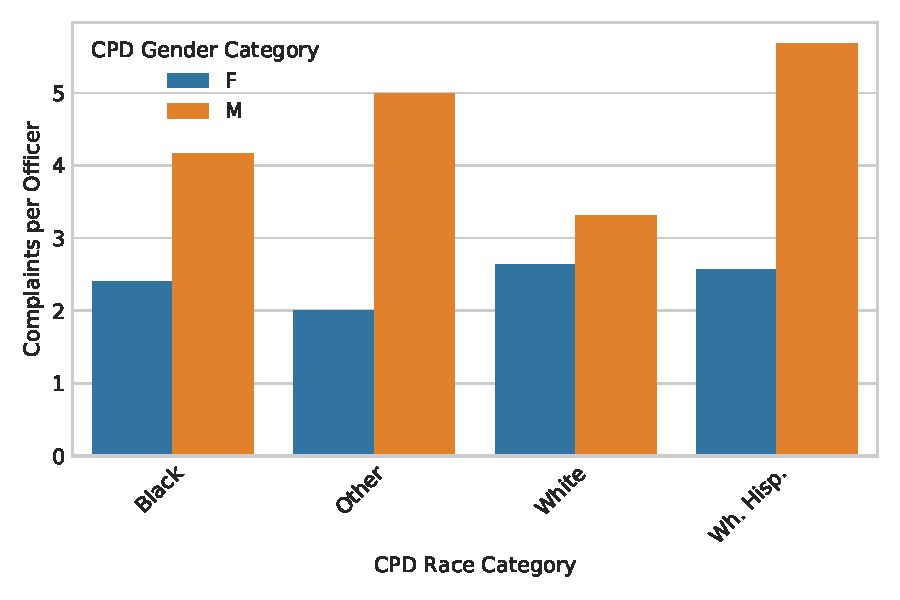
\includegraphics[width=\textwidth]{figs/complaints} 
	\caption{Temporal data for complaints.} \label{fig:complaints}
\end{figure}

We report in \Cref{fig:complaints} temporal information about complaints filed against the CPD. Interestingly, fewer complaints get filed during the weekends (although, the number of TRRs is higher then --- see \Cref{fig:trrs_times}). Moreover, complaints tend to be higher in the warmer months. Last, we notice that the number of complaints filed kept reducing over the years --- potentially as a consequence of the perception of ineffectiveness of such complaints.

\paragraph{Tactical Response Reports.}

\begin{figure}[h] 
	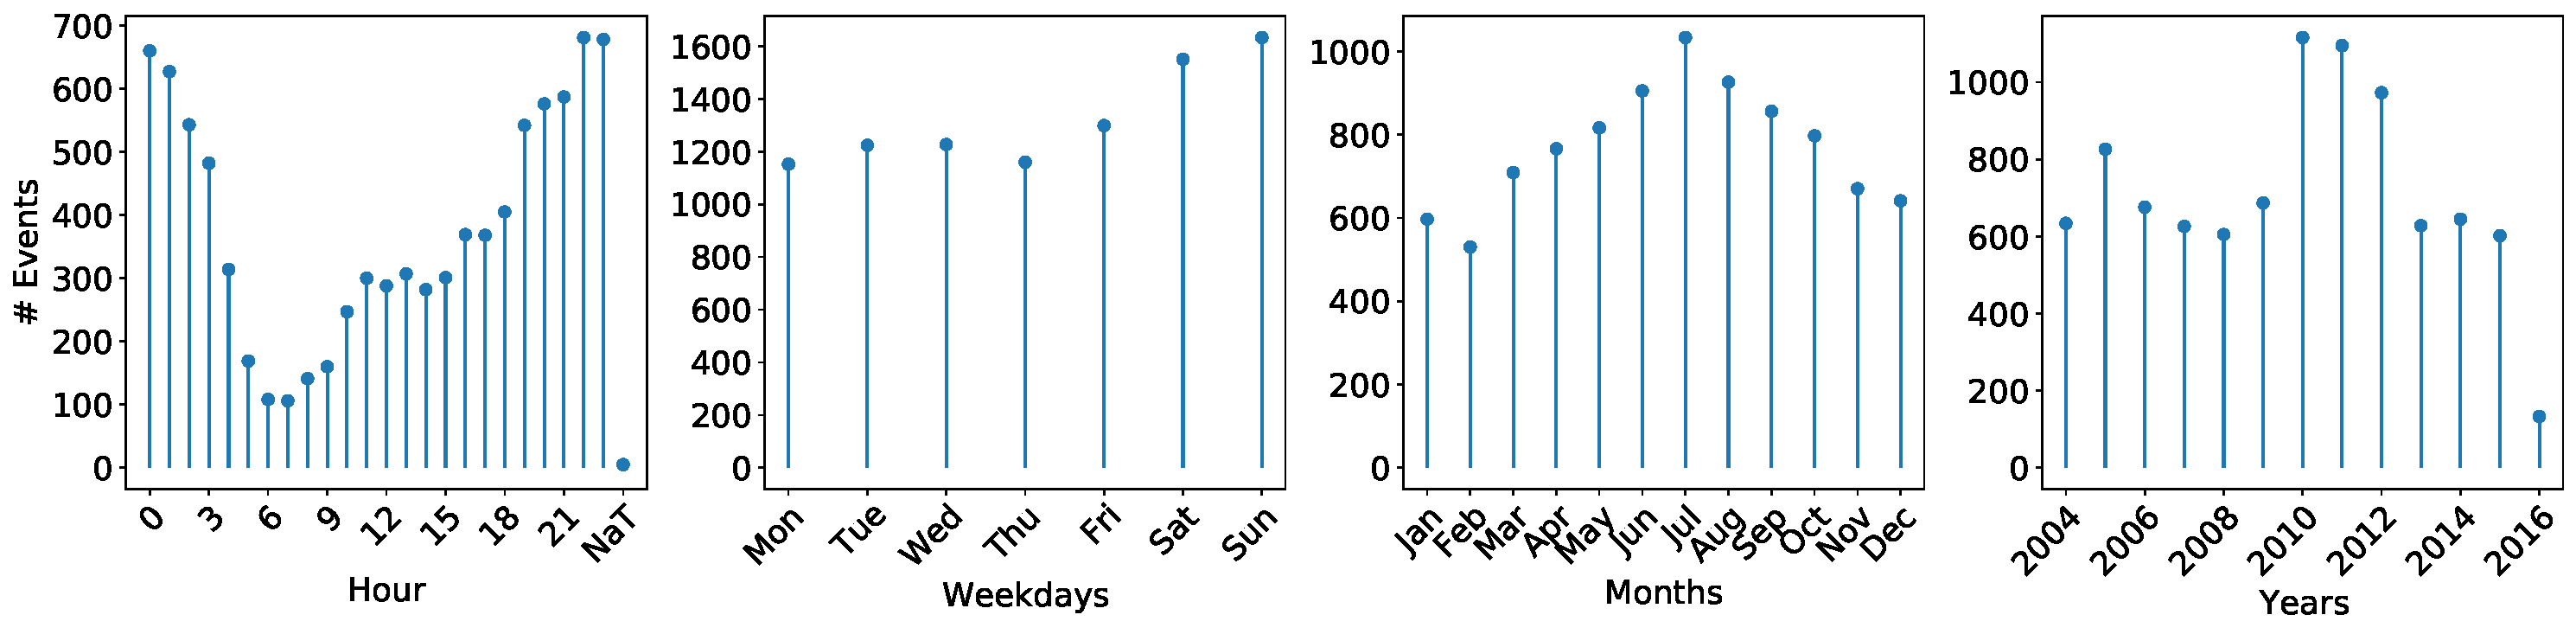
\includegraphics[width=\textwidth]{figs/trrs_times} 
	\caption{Temporal data for TRRs. Left: time during the day; mid-left: time during the week; mid-right: month; right: year.} \label{fig:trrs_times}
\end{figure}

\begin{figure}[h] 
	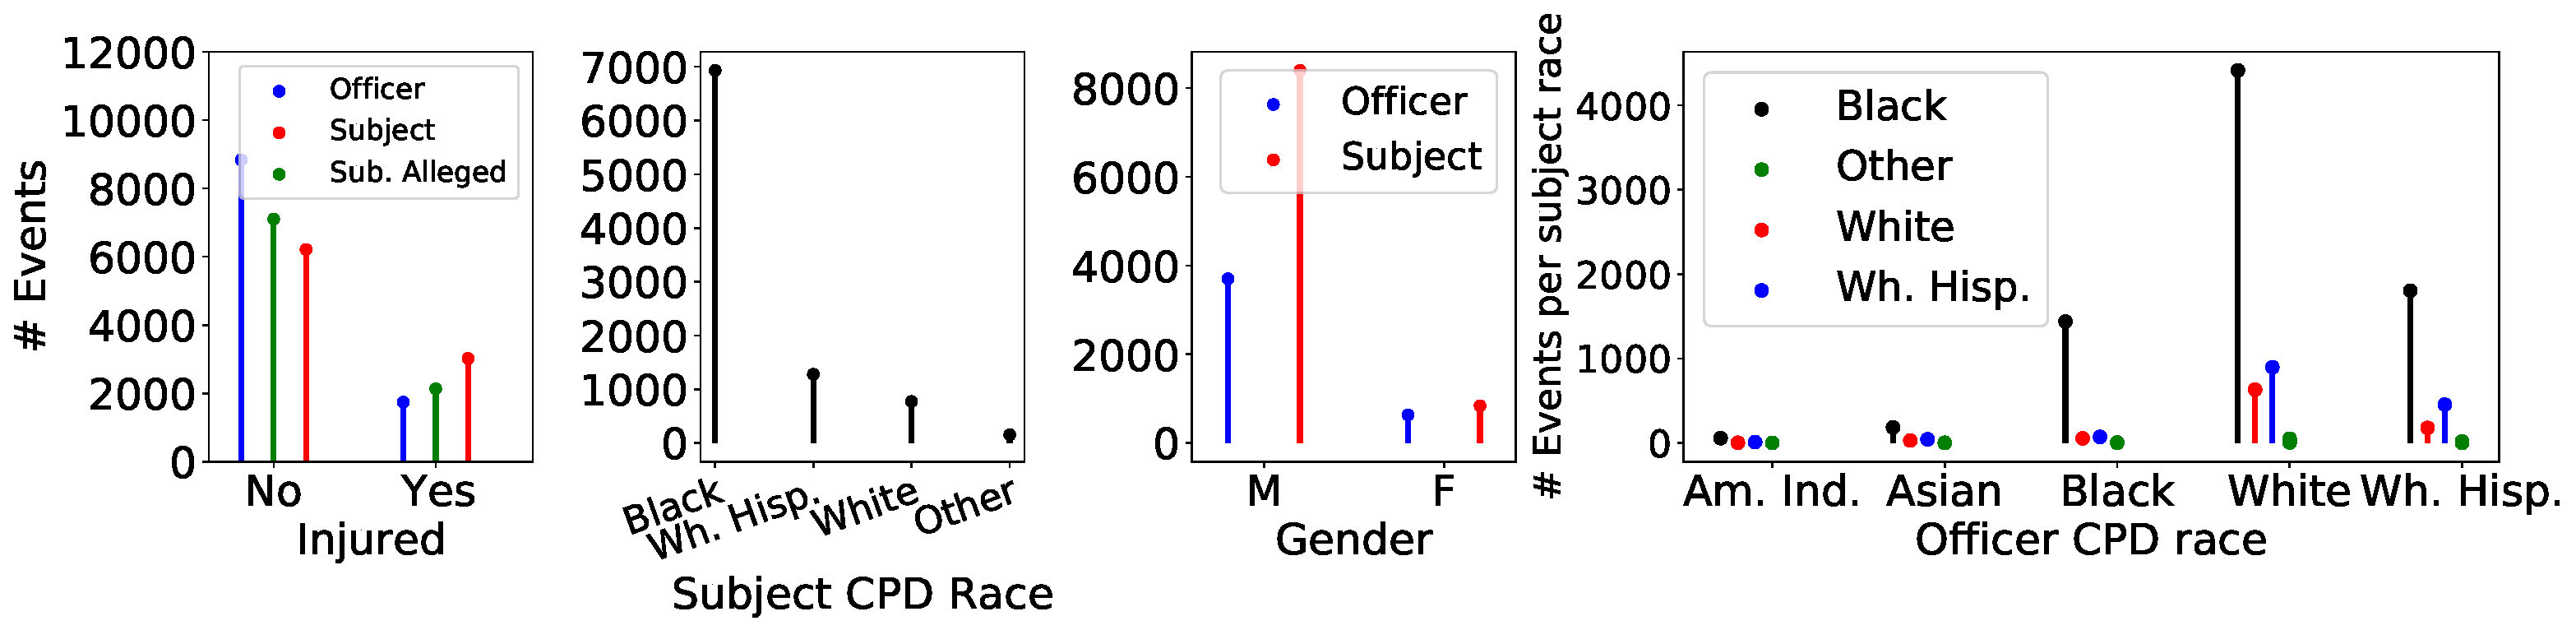
\includegraphics[width=\textwidth]{figs/trr_stats} 
	\caption{Additional statistics for TRRs.} \label{fig:trrs_stats1}
\end{figure}

%\begin{figure}[h] 
%	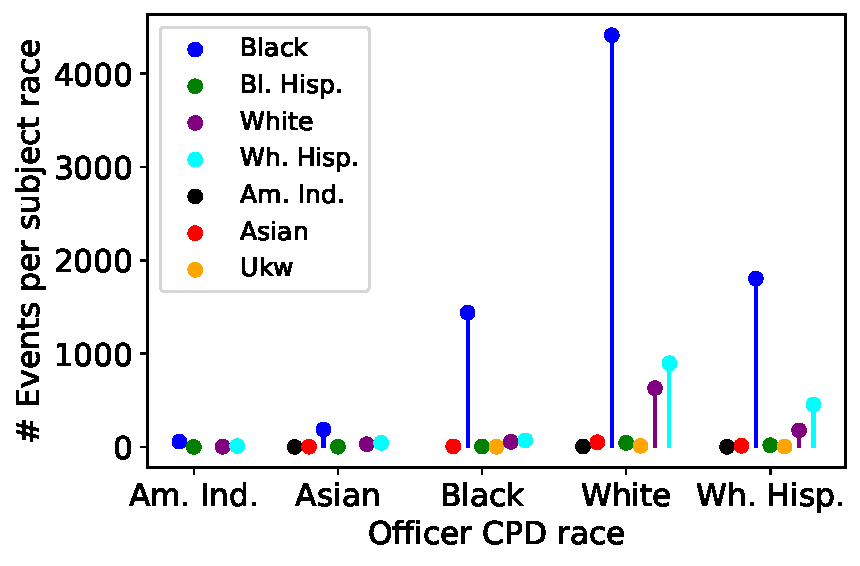
\includegraphics[width=\textwidth]{figs/trr_stats_race_race} 
%	\caption{Temporal data for TRRs.} \label{fig:trrs_stats2}
%\end{figure}

We also report temporal information about the TRRs in \Cref{fig:trrs_times}. TRRs tend to be filed more frequently at night, in the weekends, and during warmer months. Moreover, 2010, 2011 and 2012 are the years in which the highest number of TRRs have been filed. We also report in \Cref{fig:trrs_stats1} additional information about TRRs: in most cases, neither the officers nor the subjects involved get injured, although civilians get injured at a much higher rate (left subplot), and officers tend to fire first. 
\paragraph{Salary.} todo

\begin{figure}[h] 
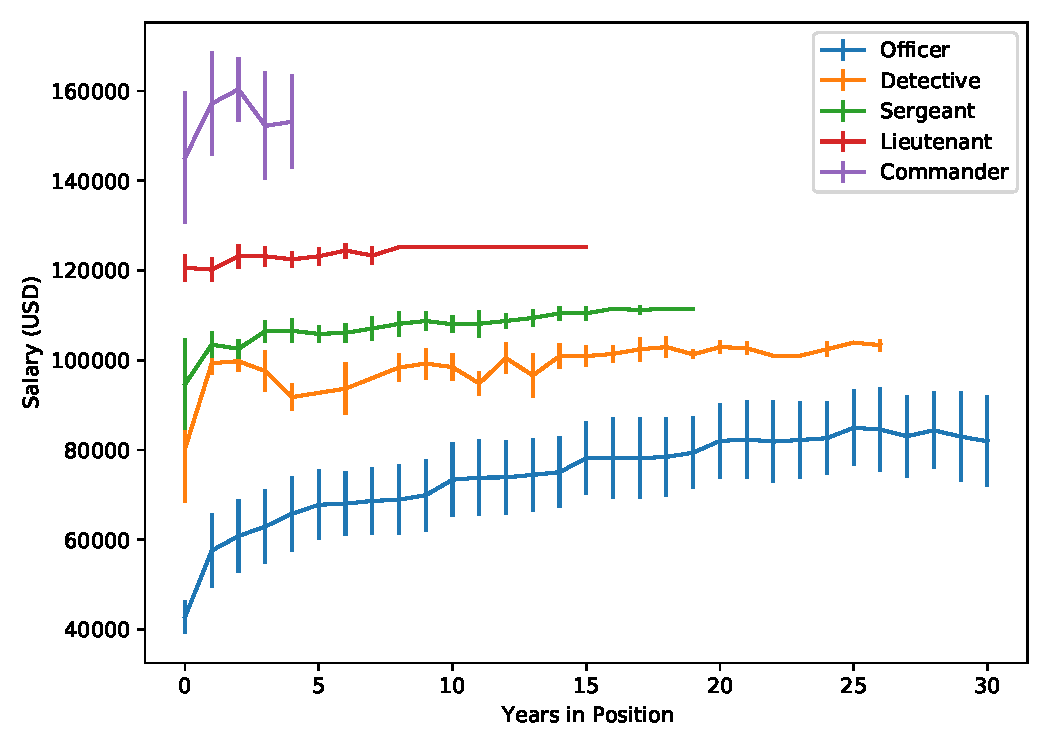
\includegraphics[width=\textwidth]{figs/salary} 
\caption{Historical data from the CPD. Salary versus experience in each
position, years x axis, salary (USD) y axis, for a few of the most common
positions. Lines are means, bars indicate 1 std dev above and below.} \label{fig:salary}
\end{figure}

\begin{figure}[h] 
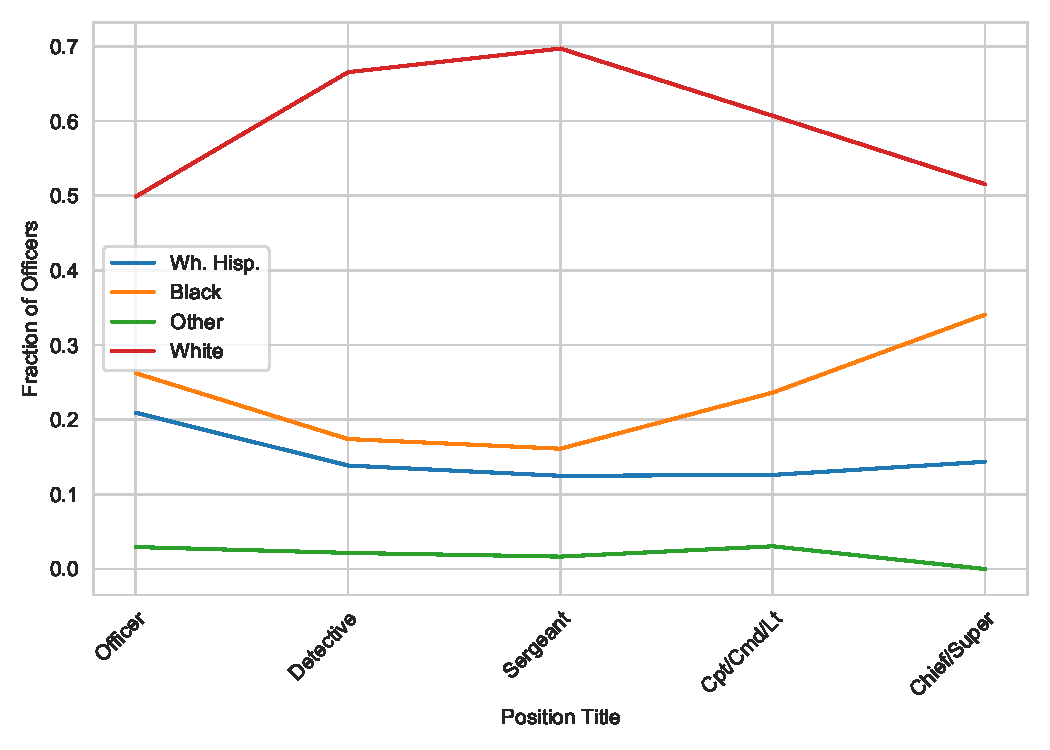
\includegraphics[width=\textwidth]{figs/position_race} 
\caption{Historical data from the CPD. Fraction of officers in representative positions 
per race category.} \label{fig:salary}
\end{figure}

\begin{figure}[h] 
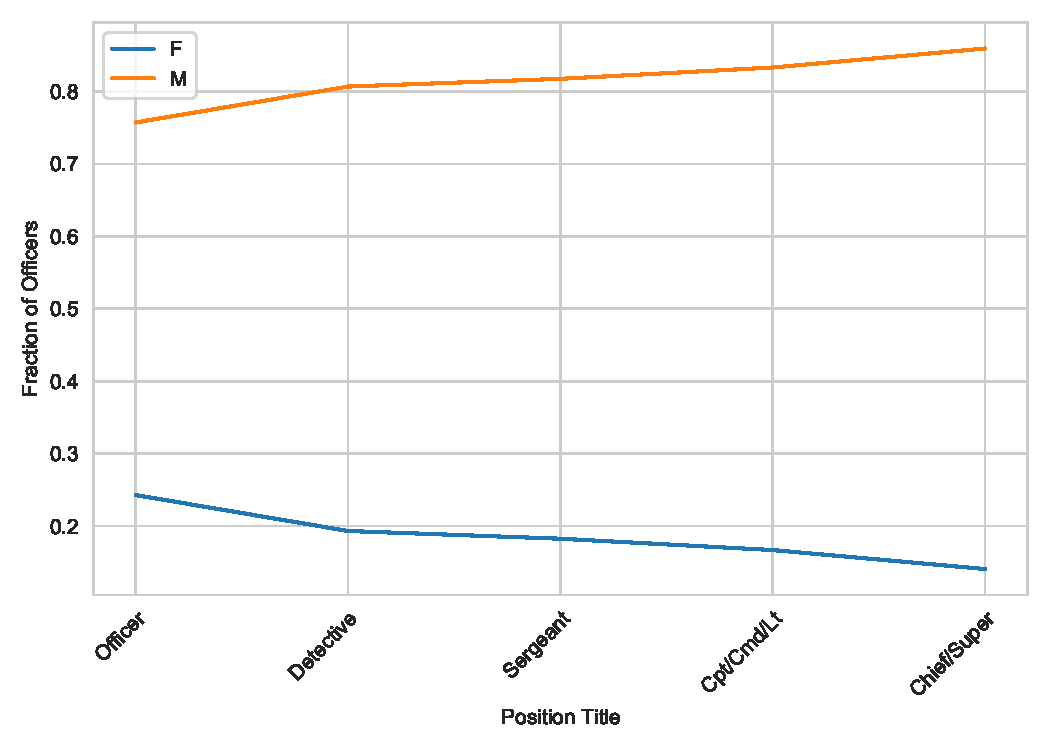
\includegraphics[width=\textwidth]{figs/position_gender} 
\caption{Historical data from the CPD. Fraction of officers in representative positions 
per gender category.} \label{fig:salary}
\end{figure}

\paragraph{Awards.}

\begin{figure}[h] 
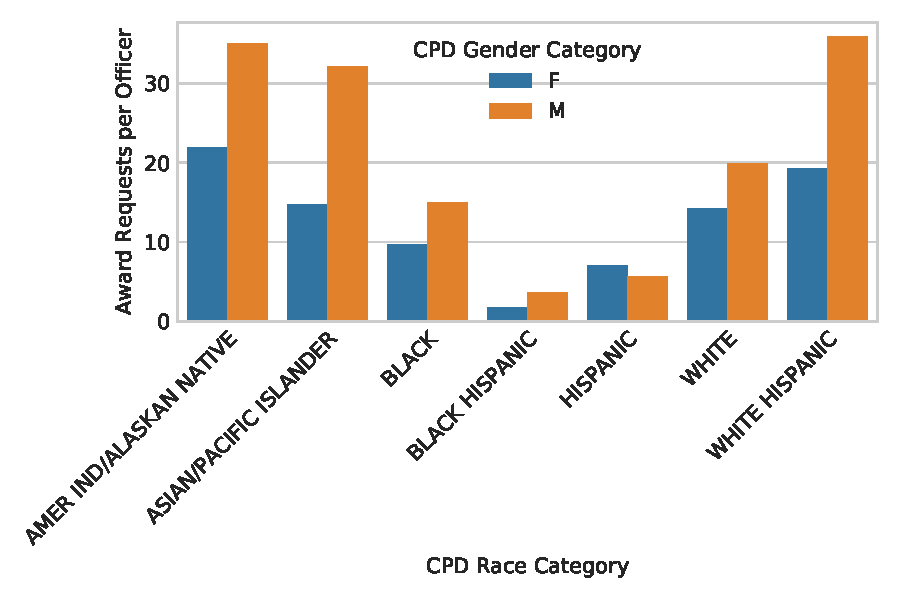
\includegraphics[width=\textwidth]{figs/awards} 
\caption{Historical data from the CPD. Awards per officer vs race for the two cpd gender categories.} \label{fig:awards}
\end{figure}




% !TEX root = ../main.tex
\section{Discussion} \label{sec:discussion}

\subsection{Intended Uses}
Uses for this dataset are varied and rich. For example, researchers could
use the data in a wide variety of predictive tasks, such as
predicting officer misconduct, resignation, and shooting as a function
of their underlying demographic data or complaints filed against them. Past work has engaged
in this type of analysis on both the raw data underlying the present
work, as well as confidential internal police department data \cite{Helsby18,Rozema19}.
This dataset can also be used to study social networks (both in the context of policing and more generally). 
In particular, we can use data in \texttt{complaints\_officers.csv} to construct an
undirected graph $\mathcal{G} = \{\mathcal{V}, \mathcal{E}\}$ in which
$\mathcal{V}$ is the set of nodes---officers appearing in at least one
complaint, and $\mathcal{E}$ the set of edges---where an edge is present
whenever two officers appear on the same complaint. Moreover, we can link the
complaints to the \texttt{tactical\_response\_reports.csv} file to consider
also the subgraph of officers who filed a TRR. We report summary statistics
for the corresponding graphs in \Cref{tab:stats_graphs}, with additional related visualizations
in \cref{sec:additional_figs}.
These networks are of interest in and of
themselves, but can also be used to investigate the dynamic patterns of officer
wrongdoing along such police networks \cite{Roithmayr16}. Existing research has used the complaint
data to identify such patterns and to investigate whether pairs of officers
connected on a network are more likely to have been accused of misconduct \cite{Ouellet19}.
Finally, this dataset could be used to track the effects of new disciplinary
practices, new training techniques, and new oversight on complaints and use of
force. A working paper explores, for example, whether civilians filed fewer
complaints about officers' force in the wake of the Department of Justice
investigation of the Chicago Police Department \cite{Travers20}. 


\begin{table}[t!]
\caption{Summary statistics for the complaints network graph, and the subgraph
of officers in TRRs. All complaints and TRRs filed between 
2004-01-01 and 2015-12-01 are considered in the network construction.
Here LCC is the largest connected component, and Is.~nodes is 
the number of isolated nodes. 
}\label{tab:network}
\begin{tabular}{c|c|c|c|c|c|c|c|}
\cline{2-8}
                                                & $|\mathcal{G}|$ & $|\mathcal{E}|$ & \textit{Avg. degree} & \textit{Triangles} & \textit{Max clique} & \textit{LCC} & \textit{\# Is. nodes} \\ \hline
\multicolumn{1}{|c|}{\textit{\textbf{All}}}     & $14{,}372$      & $106{,}701$     & $14.85$              & $361{,}878$        & $64$                & $13{,}950$   & $0$                   \\ \hline
\multicolumn{1}{|c|}{\textit{\textbf{In TRRs}}} & $4{,}105$       & $22{,}064$      & $10.75$              & $44{,}786$         & $28$                & $3{,}822$    & $225$                 \\ \hline
\end{tabular} \label{tab:stats_graphs}
\end{table}

\subsection{Ethical Considerations}
Recent work on algorithmic fairness focuses on the potential for racially
biased data to produce racially biased results
\cite{veale2018fairness,sloane2019ai,d2020fairness}.  This research suggests
that race shapes data collection in criminal justice, in at least two ways that
are likely to affect data collection on black officers. First, beginning back
in the 1960s, black officers are more likely to be assigned to black
neighborhoods and/or to neighborhoods where police interaction is more
pervasive \cite{Kuykendall80}. Given an increased frequency of interaction,
officers assigned to these neighborhoods may be statistically more likely to be
the subject of complaints \cite{Kane06}.  Second, owing to cognitive bias, complainants 
may be more likely to file a complaint against black officers, either alone or in pairs.
\cref{fig:complaints} provides initial quantitative evidence towards that point. This racial
asymmetry in the collection of complaint data may well produce, for example,
racially biased predictions of police misconduct. Relatedly, because our
dataset may be used to explore predictive policing of the police, black
officers may be unfairly and disproportionately identified to be at higher risk
of misconduct \cite{veale2018fairness,sloane2019ai,d2020fairness,Wood19}. 

\subsection{Limitations and Future Work}
Using civilian and administrator complaint data to study actual (not merely
perceived) police misconduct inevitably faces significant questions about
validity. At least one study has found that because of flaws in police record
keeping and categorization, the practice of using complaints to measure police
behavior is unreliable \cite{Hickman16}. Even so, other research finds a strong
correlation between civilian-filed complaints against officers and internal
complaints against the same officers filed by other officers or supervisors
\cite{Lersch00}. Whatever the truth of the matter, the dataset could be
strengthened by adding more objective measures of misconduct, for example, data
on individual officer misconduct from oversight agencies.

Use of this dataset for network research faces a particular set of limitations.
To wit, researchers who use complaint data to generate social networks must
acknowledge that the co-listing of two officers on a complaint is an
 incomplete proxy for a professional network relationship or
exposure to another officer's misconduct. Data on partner assignment and
dispatches would more accurately reflect officer relationships and their
exposure to misconduct. 

In general, future work should focus on integrating into this dataset as many
objective sources of data on individual officers as possible. Objective data
could include information about adverse incident histories, officer discipline
histories, counseling interventions, domestic violence incidents, weapons
violations, sustained complaints, and lawsuit settlements. Additional information
about officer activities could include partner assignments, dispatch
information, arrest and stop information, unit leadership, and unit disciplinary history. 


\section*{Acknowledgments}
T. Campbell was supported by a National Sciences and Engineering Research Council of Canada (NSERC) Discovery Grant and an NSERC Discovery Launch Supplement.

\bibliographystyle{unsrtnat}
\bibliography{references}

\section*{Checklist}

%%% BEGIN INSTRUCTIONS %%%
The checklist follows the references.  Please
read the checklist guidelines carefully for information on how to answer these
questions.  For each question, change the default \answerTODO{} to \answerYes{},
\answerNo{}, or \answerNA{}.  You are strongly encouraged to include a {\bf
justification to your answer}, either by referencing the appropriate section of
your paper or providing a brief inline description.  For example:
\begin{itemize}
  \item Did you include the license to the code and datasets? \answerYes{See Section~\ref{gen_inst}.}
  \item Did you include the license to the code and datasets? \answerNo{The code and the data are proprietary.}
  \item Did you include the license to the code and datasets? \answerNA{}
\end{itemize}
Please do not modify the questions and only use the provided macros for your
answers.  Note that the Checklist section does not count towards the page
limit.  In your paper, please delete this instructions block and only keep the
Checklist section heading above along with the questions/answers below.
%%% END INSTRUCTIONS %%%

\begin{enumerate}

\item For all authors...
\begin{enumerate}
  \item Do the main claims made in the abstract and introduction accurately reflect the paper's contributions and scope?
    \answerTODO{}
  \item Did you describe the limitations of your work?
    \answerTODO{}
  \item Did you discuss any potential negative societal impacts of your work?
    \answerTODO{}
  \item Have you read the ethics review guidelines and ensured that your paper conforms to them?
    \answerTODO{}
\end{enumerate}

\item If you are including theoretical results...
\begin{enumerate}
  \item Did you state the full set of assumptions of all theoretical results?
    \answerTODO{}
	\item Did you include complete proofs of all theoretical results?
    \answerTODO{}
\end{enumerate}

\item If you ran experiments (e.g. for benchmarks)...
\begin{enumerate}
  \item Did you include the code, data, and instructions needed to reproduce the main experimental results (either in the supplemental material or as a URL)?
    \answerTODO{}
  \item Did you specify all the training details (e.g., data splits, hyperparameters, how they were chosen)?
    \answerTODO{}
	\item Did you report error bars (e.g., with respect to the random seed after running experiments multiple times)?
    \answerTODO{}
	\item Did you include the total amount of compute and the type of resources used (e.g., type of GPUs, internal cluster, or cloud provider)?
    \answerTODO{}
\end{enumerate}

\item If you are using existing assets (e.g., code, data, models) or curating/releasing new assets...
\begin{enumerate}
  \item If your work uses existing assets, did you cite the creators?
    \answerTODO{}
  \item Did you mention the license of the assets?
    \answerTODO{}
  \item Did you include any new assets either in the supplemental material or as a URL?
    \answerTODO{}
  \item Did you discuss whether and how consent was obtained from people whose data you're using/curating?
    \answerTODO{}
  \item Did you discuss whether the data you are using/curating contains personally identifiable information or offensive content?
    \answerTODO{}
\end{enumerate}

\item If you used crowdsourcing or conducted research with human subjects...
\begin{enumerate}
  \item Did you include the full text of instructions given to participants and screenshots, if applicable?
    \answerTODO{}
  \item Did you describe any potential participant risks, with links to Institutional Review Board (IRB) approvals, if applicable?
    \answerTODO{}
  \item Did you include the estimated hourly wage paid to participants and the total amount spent on participant compensation?
    \answerTODO{}
\end{enumerate}

\end{enumerate}


\appendix

\section{Datasheet}\label{sec:datasheet}

This section provides a datasheet \cite{Gebru18} for the dataset repository.

\subsection{Motivation}

\paragraph{For what purpose was the dataset created?}
The original raw data files were sought by J.~Kalven, a journalist in the City
of Chicago, as part of his investigation into police abuse. After the original
FOIA requests and legal case, the non-profit Invisible Institute (\url{https://invisible.institute}) 
began to collaborate with Kalven and the University of Chicago's Mandel Legal Aid Clinic
to follow up on earlier FOIA requests and to file new ones. The data disclosed
in response to these earlier and now ongoing FOIA requests were made available
online as part of the Citizens Police Data Project.

\paragraph{Who created the dataset, and on behalf of which entity?}
The Chicago Police Department (CPD), Civilian Office of Police Accountability
(COPA), and the City of Chicago produced the raw data files in response to FOIA
requests. The raw data were curated and released publicly by the Invisible
Institute and its collaborators. The cleaned and linked data were produced
as part of research by the authors of this document.

\paragraph{Who funded the creation of the dataset?}
The acquisition of the original raw data was funded by the Invisible Institute.

\subsection{Composition}

\paragraph{What do the instances that comprise the dataset represent?}
There are multiple types of instance in this data. 
\begin{itemize}
\item Officer: information about an individual police officer
\item Unit assignment: a single unit assignment for an officer
\item Complaint: a complaint filed against a police officer, either internally or by a civilian
\item Tactical Response Report: a form that an officer is required to fill out after their response requires use of force
\item Award request: a request to grant an award to an officer
\item Salary: a record of an officer's salary, pay grade, and position across multiple years
\end{itemize}

\paragraph{How many instances are there in total (of each type)?}
There are roughly 35,000 unique officers in the cleaned roster appearing in roughly 130,000 profiles throughout the data,
730,000 award request records,
194,000 salary records,
108,000 unit assignment records,
109,000 complaints,
and 10,500 tactical response reports.

\paragraph{Does the dataset contain all possible instances or is it a sample of instances from a larger set?}
This data contains information regarding all sworn officers in the Chicago Police Department / City of Chicago
databases for the stated date ranges (which differ for each source of raw data).

\paragraph{What data does each instance consist of?}
\begin{itemize}
\item Officer: officer unique ID, race, gender, age, appointment date, resignation date, badge number(s), position title(s)
\item Unit assignment: officer unique ID, start date, end date, unit number
\item Complaint: complaint ID, involved officer IDs, allegation, result of the investigation, resulting sanction (where available)
\item Tactical Response Report: report ID, event location, date, and time, environmental conditions, who was notified, weapons discharged, weapon information, subject demographic information 
\item Award Request: awardee unique ID, requester, request date, award reference number, award type, request tracking number, incident dates, ceremony date
\item Salary: officer unique ID, salary, position title, pay grade, year
\end{itemize}

\paragraph{Is there a label or target associated with each instance?}
Not explicitly. However, labels could be constructed from the data 
that exists. For example, one could aggregate complaints to produce
an integer ``number of complaints'' for each officer in the data,
and use that as the response variable in a prediction task.

\paragraph{Is any information missing from individual instances?}
In the original raw data files, missing data (of all fields) is quite common.
In the cleaned and linked data files, we are able to aggregate multiple profiles
of a single officer appearing throughout the data to ``fill in the gaps,'' although
this process is not perfect and there are still missing entries.

\paragraph{Are relationships between individual instances made explicit?}
In the raw data, no. In the cleaned data, we provide a unique officer
identification that enables linking the activities and records regarding
individual officers across datasets. There is no relational data (i.e., network edges)
explicitly contained in the data. However, it is possible to use the data
to construct a network, e.g., by linking officers co-listed on complaints.

\paragraph{Are there recommended data splits?}
No.

\paragraph{Are there any errors, sources of noise, or redundancies in the dataset?}
There are redundancies in the raw data, but these are removed by our cleaning and linking procedure.
Errors, inconsistencies, and missing data are also present in the raw data; our cleaning and linking
resolves much of these issues. However, per \cref{sec:analysis}, the officer database is
likely to be incomplete prior to roughly 1980 (as officers were added to the database only gradually over time).

\paragraph{Is the dataset self-contained, or does it rely on external resources?}
The dataset is self-contained: the raw data itself is stored in the \url{raw/} folder of the repository 
(with links to the external source files for reference), 
and the cleaned/linked data is produced by the source code in the repository.

\paragraph{Does the dataset contain data that might be considered confidential?}
No; all of this data was publicly released as part of FOIA requests. 
Confidential data (e.g., relating to under cover officers) was withheld 
by the Chicago Police Department.

\paragraph{Does the dataset contain data that, if viewed directly, might be offensive, insulting, or threatening?}
No.

\paragraph{Does the dataset relate to people?} 
Yes; it contains records relating to police officers in the Chicago Police Department.

\paragraph{Does the dataset identify any subpopulations?}
Yes; officer records include race, gender, age, appointment date, unit history, badge numbers, position title,
salary, awards, complaints, and tactical response reports. Subpopulations of officers can be constructed
using these fields.

\paragraph{Is it possible to identify individuals?}
Yes; detailed information is available that could be used to identify individual officers.

\paragraph{Does the dataset contain data that might be considered sensitive in any way?}
The data contains a coarse categorization of racial origins of officers.

\subsection{Collection Process}

\paragraph{How was the data associated with each instance acquired?}
The raw data were obtained via FOIA requests to the City of Chicago and Chicago Police Department.

\paragraph{What mechanisms or procedures were used to collect the data?}
The raw data were obtained via FOIA requests to the City of Chicago and Chicago Police Department.

\paragraph{If the data are a sample from a larger set, what was the sampling strategy?}
Not applicable. 

\paragraph{Who was involved in the data collection process and how were they compensated?}
Journalists in collaboration with the Invisible Institute were responsible for filing
the FOIA requests, and officials within the Chicago Police Department and City of Chicago were responsible
for providing data in response to those requests. It is not known explicitly whether or how 
either party was compensated.

\paragraph{Over what timeframe was the data collected?}
The earliest releases per FOIA request occurred in 2016, and continue to occur
as more FOIA requests are filed. The raw data itself pertain to records from the CPD
dating back to the mid 20th century. The roster data covers the period up
to 2018. The awards data pertains to records from 1967 to 2019.
The salary data pertains to the years 2002 to 2017. The unit history data covers records up
to 2016. The complaints data pertains to records from 1967 to 2016. The tactical response 
report data pertains to records from 2004 to 2017.

\paragraph{Were any ethical review processes conducted?}
It is unknown whether the CPD conducted any ethical review processes prior to the release
of the raw data. No ethical review process was conducted prior to the activities
involved in the present repository, i.e., cleaning the publicly available data.

\paragraph{Does the dataset relate to people?}
Yes; it contains detailed records regarding the activities of police officers in the City of Chicago.

\paragraph{Did you collect the data from the individuals directly, or obtain it via third parties?}
The raw data was acquired from public links provided by the Invisible Institute (\url{https://invisible.institute}).
The Invisible Institute acquired the data through FOIA requests made to the CPD and the City of Chicago.

\paragraph{Were the individuals notified about the data collection?}
It is unknown whether the individual officers were notified by the CPD when the raw data was released. 

\paragraph{Did the individuals in question consent to the collection and use of their data?}
Not explicitly. The Chicago Police Department was compelled by law to produce these records per FOIA requests.

\paragraph{If consent was obtained, were the consenting individuals provided with a mechanism to revoke their consent in the future or for certain uses?}
Not applicable.

\paragraph{Has analysis of the potential impact of the dataset and its use on data subjects been conducted?}
Not known.

\subsection{Preprocessing and cleaning}

\paragraph{Was any preprocessing of the data done?}
Yes; the main section of this documentation provides details the cleaning and linking of the raw
data resulting from FOIA requests made to the City of Chicago.

\paragraph{Was the ``raw'' data saved in addition to the cleaned data?}
Yes; the raw data is available in the \url{raw/} folder in the repository.

\paragraph{Is the software used to clean the data available?}
Yes; the source for cleaning and linking is provided in the \url{src/} folder in the repository.

\subsection{Uses}

\paragraph{Has the dataset been used for any tasks already?}
Not the newly cleaned and linked version.
The raw data itself has been used previously; see \cref{sec:discussion} for details.

\paragraph{Is there a repository that links to any or all papers that use the dataset?}
Not that the authors of this work are aware of.

\paragraph{What (other) tasks could the dataset be used for?}
This data set has a rich variety of possible uses; for example,
network analysis (and in particular, analysis of dynamic events occurring on networks)
and predictive regression/classification. See \cref{sec:discussion} for more details.

\paragraph{Is there anything about the composition of the dataset or the way it was collected and cleaned that might impact future uses?}
Yes; the data are less reliable in earlier years (e.g., pre-1980). See \cref{sec:analysis} for more details.

\paragraph{Are there tasks for which the dataset should not be used?}
This data should not be used to single out, study, or identify individual officers.

\subsection{Distribution}

\paragraph{Will the dataset be distributed to third parties outside of the entity on behalf of which the dataset was created?}
Yes, the data is publicly available.

\paragraph{How will the dataset be distributed?}
It is available on GitHub at \url{https://github.com/chicago-police-violence/data}.
Release versions will be marked using the ``release'' feature on GitHub.

\paragraph{When will the dataset be distributed?}
It is currently publicly accessible.

\paragraph{Will the dataset be distributed under a copyright, other IP license, or terms of use?}
Yes; the source code is released under the MIT license, and the data output by the cleaning code is released under the Creative Commons 4.0 BY-NC-SA license.

\paragraph{Have any third parties imposed IP-based or other restrictions on the data associated with the instances?}
No.

\paragraph{Do any export controls or other regulatory restrictions apply to the data?}
No.

\subsection{Maintenance}

\paragraph{Who is supporting/hosting/maintaining the dataset?}
The repository will be hosted on GitHub. As of August 2021, the repository
owners are Thibaut Horel, Trevor Campbell, and Lorenzo Masoero, but ownership
may change over time.

\paragraph{How can the data owner/curator be contacted?}
Issue threads on GitHub are the primary channel of contact for the repository maintainers.

\paragraph{Is there an erratum?}
Not as of yet. For each major release version, notes will be included and
hosted in the repository that will detail cleaning/linking errors that have been fixed.

\paragraph{Will the dataset be updated?}
The original raw source data from FOIA requests will not be modified. More raw
data files may be added over time corresponding to new FOIA requests. The data
cleaning and linking code will be edited over time to fix errors; release
versions will be clearly marked on GitHub. There is no set schedule for updates.

\paragraph{If the dataset relates to people, are there applicable limits on the retention of data associated with the instances?}
No; this data was released per FOIA requests and is in the public domain.

\paragraph{Will older versions of the dataset continue to be supported/hosted/maintained?}
Yes; a full version-controlled history of the project exists on GitHub.

\paragraph{If others want to extend/augment/build on/contribute to the dataset, is there a mechanism for them to do so?}
Yes; the repository for the dataset is hosted on GitHub, where pull requests are a usual channel for external contribution.

\section{Data Cleaning and Linking: Additional Details}\label{sec:app-cleaning}

\subsection{Initial Cleaning}

The files initially released by the CPD are for
the most part Excel spreadsheets, with inconsistent formatting and which can
thus be difficult to process programmatically. As an example, the reader is
invited to open the file
\texttt{p046957\_-\_report\_1.1\_-\_all\_complaints\_in\_time\_frame.xls}
available in the folder \texttt{raw/P0-46957/}. As can be seen, each record in
this file is spread over two rows of the spreadsheet, with the field names
repeated at the beginning of the second row for each record.

Consequently, the goal of the cleaning step is to produce uniformly formatted
CSV files, with the minimum requirement that each record be presented on
a single line after this step. The code is contained in the files
\texttt{datasets.py}, \texttt{parse.py}, \texttt{parse\_p046957.py}, and \texttt{parse\_p061715.py} in the
\texttt{src/} folder.  The step can be applied by running \texttt{make prepare}
in the root of the repository, which creates the folder \texttt{tidy/}
containing the cleaned CSV files.

The decisions made at this stage are straightforward and involve no subjective
judgment. They consist of:
\begin{itemize}
	\item Unifying attribute names across datasets, so that the same type of
		data is always identified in the same way (for example,
		\texttt{Appointment Date}, \texttt{Appt Date},
		\texttt{appointment\_date} are all mapped to
		\texttt{appointment\_date}).
	\item Unifying attribute values across datasets. For example, the gender of
		an officer is indicated as a single letter \texttt{M}/\texttt{F} in
		some datasets, and as \texttt{Male}/\texttt{Female} in others. A similar issue
		arises with the race of officers, sometimes given as a three-letter
		code, and sometimes described in full. In such cases we map all
		possible forms of an attribute value to a canonical one. \footnote{Probably for space, can merge these two bullet points as ``Unifying attribute names and values across datasets''.}
	\item Parsing values into the correct data type or format. For example,
		dates and times are formatted differently depending on the dataset, and
		we map everything to the ISO\,8601 format. Integers are also parsed so
		as to remove the various paddings present in the original data.
	\item Concatenating all the files containing a given type of record in each
		data release. Indeed, the CPD's responses to some FOIA requests split
		the records chronologically over multiple Excel spreadsheets (see for
		example \texttt{raw/P0-46957}) or multiple tables within spreadsheets
                (see for example \texttt{raw/salary}). Having a single file for each record
		type instead simplifies later processing steps.
\end{itemize}

Although this initial cleaning is only the first step in the process producing
our final dataset, we structured our processing code in such a way that it is
easy to stop the process at this step and keep the intermediate output in the
\texttt{tidy/} folder. This is because the next steps required making more
subjective judgment calls, e.g., to decide how to clean erroneous records and resolve
ambiguities arising from the merging and linking of datasets. Consequently, it
is possible that some applications will require performing these next steps
differently. In such cases, the files contained in the \texttt{tidy/} folder
should provide a safe intermediate point at which to branch off from our
processing pipeline.

\subsection{Linking and Merging Datasets}\label{sec:linking}
\label{sec:linking}

\paragraph{Overall description.}

As discussed in \cref{sec:raw}, the main challenge in processing the raw data
is that officers are not uniquely identified across datasets. In other words,
there is no foolproof way to know if two different records from two different
datasets correspond to the same individual. For example, a na\"ive matching
procedure identifying two officers as being the same individual whenever they
have the same name is inadequate: given the size of the CPD roster (over 35\,000
active or retired officers), it is guaranteed to contain many homonymous
individuals. Furthermore, even though the original datasets contain several
identifying attributes (name, birth year, appointment date, race, gender),
those can change over item as mentioned in \cref{sec:raw}.

At a high level, our procedure \emph{grows} a population of uniquely identified
officers by sequentially examining each FOIA release. Each unique officer in
this population is assigned a unique identification (UID), which is a random
hexadecimal string (e.g.\ \texttt{9bc51eef-c37b-4eff-a14d-7e69f56b3d1e}), and
to each UID is associated a list of \emph{officer profiles}. There is one
\emph{officer profile} for each unique officer and each FOIA release in which
this officer appeared, listing the identifying attributes of this officer as
they appear in this given data release. In detail, for each FOIA release:
\begin{enumerate}
	\item We build a list of all the \emph{officer profiles} appearing in this
		release.
	\item For each officer profile, we attempt to \emph{match} it against the
		profiles of the population of unique officers constructed so far from
		previously examined FOIA releases.
		\begin{itemize}
			\item If the match is successful, we have identified a unique officer in
				the population whose profiles unambiguously match with the
				current profile. In this case, we simply attach the current
				profile to this officer and UID, and
				the population does not grow.
			\item If the match is unsuccessful, we add a new officer with a new UID to the population of unique
				officers and attach the current profile to this new officer.
		\end{itemize}
\end{enumerate}

After all FOIA releases have been processed, the population contains the set of
all unique officers appearing in the original data. Each officer is represented
by UID and a collection of profiles, representing the various ways in which
this unique officer appears across different datasets. These profiles can be
found in the file \texttt{final/officer\_profiles.csv}.
At this point the \texttt{final/} folder also contains
one file for each type of record (complaints, tactical response reports, etc).
Within these files, officers are identified solely by their UID and other attributes
are removed; this avoids duplication of
information since these attributes are redundant with those found in
\texttt{final/officer\_profiles.csv}.

Note that this procedure depends on the order in which the FOIA releases are processed,
since each release will be matched against the profiles from all
previously considered releases. We chose to first process the two roster datasets
(\texttt{P0-58155} and \texttt{P4-41436}) since they are most similar and
supposed to contain one record for each officer in the CPD. Next, we process
the two unit assignments datasets (\texttt{16-1105} and \texttt{P0-52262})
since they are also supposed to cover the entire CPD. Finally, we process the
complaints, tactical response reports, awards, and salary data, in this
order.

\paragraph{Iterative pairwise matching.}
It remains to describe the \emph{match} operation which was left unspecified in
step 2.\ of the procedure above. This operation
matches a list of profiles found in the FOIA release being currently processed
against an already existing list of profiles and associated UIDs. We need to strike a balance between:
\begin{itemize}
	\item Being loose enough to avoid type II error (false negatives). If the
		same officer appears with slightly different attributes in two
		different profiles, we do not want the matching method to believe these
		profiles are attached to different officers.
	\item Being strict enough to avoid type I error (false positives). We do
		not want to attach a profile to an officer currently in the population
		if it in fact corresponds to a new officer.
\end{itemize}

We developed an \emph{iterative pairwise matching procedure}\footnote{This
procedure was inspired by a similar one developed by the Invisible Institute.},
that makes iterative passes over the list $L_1$ of profiles to be matched
against the list $L_2$ of already existing profiles. Recall that in our case,
the profiles in $L_2$ are associated with officers in the growing population of
unique officers, and hence they are each associated with a UID. During each
pass:
\begin{enumerate}
	\item A subset $S$ of the profile attributes is selected as the matching
		criterion.
	\item For each profile $p$ in $L_1$:
		\begin{enumerate}
			\item Construct the list $\ell_p$ of profiles in $L_2$ for which
				the attributes in $S$ match with $p$ exactly.
			\item If all the profiles in $\ell_p$ are associated with the same
				UID $u$, this is an unambiguous match and we can safely assign
				the UID $u$ to the profile $p$. We remove $p$ from $L_1$ and
				all the profiles associated with $u$ in $L_2$.
			\item Otherwise, the match is ambiguous and we keep $p$ in
				$L_1$.
		\end{enumerate}
\end{enumerate}
Observe that both $L_1$ and $L_2$ decrease in size as matches are found, so
each pass iterates over a smaller set of profiles than the previous one. When
all passes are done, the remaining profiles in $L_1$ are considered new
unique officers and assigned freshly generated UIDs. Furthermore, by
building at each pass a hash table mapping a subset of attributes to the
list of profiles in $L_2$ sharing these attributes, the construction of
$\ell_p$ in 2.(a) can be performed in constant time. The overall running time of the
  iterative matching procedure is $O\big(P(|L_1|+|L_2|)\big)$ where $P$ is the
  number of passes.\footnote{\textcolor{red}{If we are talking about running time, I think we could also mention that - in practice - this procedure runs in less than a minute (or actually, check how long it takes) on a standard machine?}}

Finally, to fully specify the matching procedure we need to describe how to
choose which subset $S$ of identifying attributes is chosen as the matching
criterion at step 1.\ during each pass. For this, we go from the stricter to
the looser criterion: in the first pass, $S$ contains \emph{all} the attributes
which are present in both $L_1$ and $L_2$, and then attributes are removed from
$S$ one by one in subsequent passes. For example, one can remove the \emph{last
name} attribute in the second pass to match a pair of profiles whose last names
are different but match on all the remaining attributes, thus identifying an
officer whose last name changed between two FOIA releases. The advantage of
going from stricter to looser is twofold:
\begin{itemize}
	\item Starting from the strictest set of attributes identifies the
		\emph{least ambiguous matches}, for which profiles match exactly on
		a large set of attributes and can confidently be considered to describe
		the same individual. This constitutes the vast majority of cases;
		more than 95\% of profiles are usually matched during the first pass.
		Since the next passes iterate only on the remaining profiles, this
		removes the majority of ambiguities that could arise as the
		matching criterion is relaxed.
	\item Since the vast majority of profiles are matched in the first pass,
		it becomes feasible in subsequent passes to visually inspect all
		the matched profiles and assess whether the chosen set of attributes was
		too strict or too lose.
\end{itemize}

We note that there is some amount of subjective judgement involved;
 visual inspection is employed in the second and subsequent passes to decide which sets
attributes are stringent enough as to avoid accidentally matching two different persons. 
This is also how we decide that sufficiently many passes have been
performed and that further relaxing the matching criterion would introduce too
many type I errors. In general, we erred on the side of favoring
type II errors over type I errors when uncertain.

%\textbf{TODO:} explain the few subtleties where we don't use equality to match
%attributes (for example when matching age and birthyear, where the age only
%lets us identify the birthyear with an accuracy of 1 year). Or with stars,
%where we test whether a star number is contained in the subset of known stars
%for this officer.

%\textbf{TODO:} table of officer attributes in each dataset


\subsection{Final cleaning and output}

\paragraph{Roster consolidation.}
The procedure described in \cref{sec:linking} produces, for each unique officer
in our dataset, a collection of profiles presenting the list of identifying
attributes of this officer as they appear in each dataset provided by the CPD.
Since these attributes can change over time for legitimate reasons, we believe
that the collection of profiles as a whole is the most faithful and complete
representation of each officer. Working with such collections of profiles can
however be counter-intuitive and inconvenient, since some applications might
for example require to display the name of an officer, without having to choose
from possibly two or more names in cases this officer changed name over the
course of their career in the CPD. For such use cases, we consolidated the
different profiles of each officer into a single, canonical profile as follows.
For each officer's identifying attribute, we choose the \emph{most recent
nonempty} value it takes among all profiles of this officer, where \emph{most
recent} is defined using the release date of each dataset by the CPD. In this way,
if an attribute is empty in some profiles but present in others, a nonempty value
will be selected. Choosing the most recent value is justified since (1) it is
more likely to still be current (2) it is more likely to contain the latest
corrections made by the CPD to their database.\footnote{This assumes that it
is, on average, less likely for errors to be introduced in the CPD database,
than for records to be fixed. This assumption is highly debatable and the
authors' posterior belief after working on the CPD data for more than a year
assigns probability at most $0.6$ to its veracity.} The consolidated profiles
for each unique officer can be found in the file \texttt{data/roster.csv}.

\paragraph{Cleaning unit assignments.}
As already alluded to in \cref{sec:raw}, the unit assignment data revealed that
around 6\% of the records have an end date which chronologically precedes the
start date. A closer inspection of these faulty records revealed a systematic
pattern: whenever such a record appears, it is possible to find among the other
assignments of the same officer another record whose start date is exactly one
day after the end date of the faulty record. For example, displaying each
record as a triplet (\texttt{unit\_number}, \texttt{start\_date},
\texttt{end\_date}), we might find for a given officer:
\begin{quote}
\begin{verbatim}
  1 1967-12-18 1972-05-06
 22 1967-12-18 1967-12-17
\end{verbatim}
\end{quote}
where the end date for the faulty assignment to unit $22$ is one day before the
start date of the assignment to unit $1$. This led us to formulate the
following hypothesis: \emph{the faulty end dates where not manually entered but
were instead automatically generated by the data infrastructure of the CPD}.
More specifically, we believe the end dates were added by a computer code which
processed all unit assignments in order, and set as the end date of each
assignment, the day immediately preceding the start date of the following
assignment. The faulty records then arose from the fact that they were wrongly
positioned in the order considered by the computer code. The reason for the
wrong positioning of these records is that they are for the most part,
erroneous, inactive records which, we believe, should have been removed from
the dataset.

A strong supporting piece of evidence is that for 92\% of these faulty records,
we can find another record for the same officer with the same start date and
different unit number, as in the example above. An attempt at reconstructing the
true story behind this example is as follows. On 1967-12-18, someone
wrongly entered an assignment to unit $22$ for this officer, the mistake was
immediately noticed and a new, correct assignment to unit $1$ was added to the
database on the same day. When end dates were later added by the above
mentioned piece of computer code, the assignment to unit $1$ was processed
last, hence adding 1967-12-17 (the day preceding the assignment to unit $1$) as
the end date of the assignment to unit $22$. The correct solution in this case
is to simply remove the assignment to unit 22 from the dataset.

A detailed description of how the remaining 8\% of the faulty records (486
records out of the 116\,027 records in the original data) are processed can be
found in the script \texttt{src/clean\_assignments.py}.

\paragraph{Final output.}


\section{Additional summary figures}\label{sec:additional_figs}

\begin{figure}[h] 
	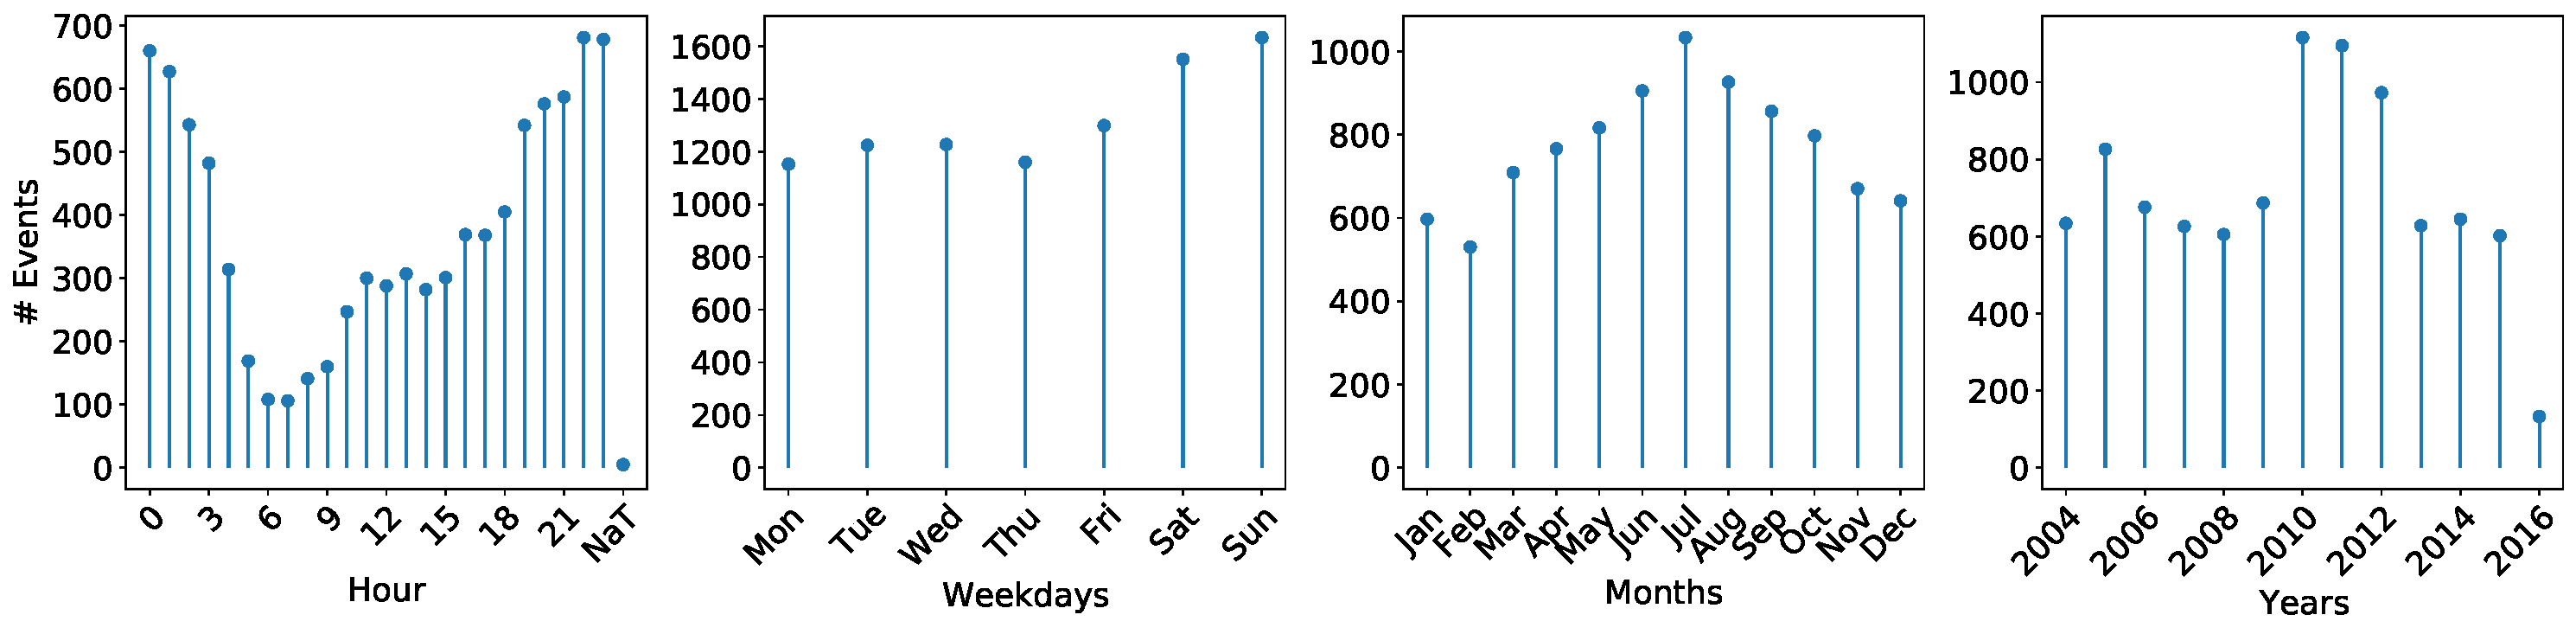
\includegraphics[width=\textwidth]{figs/trrs_times} 
	\caption{Temporal data for TRRs. Left: time during the day; mid-left: time during the week; mid-right: month; right: year.} \label{fig:trrs_times}
\end{figure}

\begin{figure}[h] 
\begin{subfigure}{0.45\textwidth}
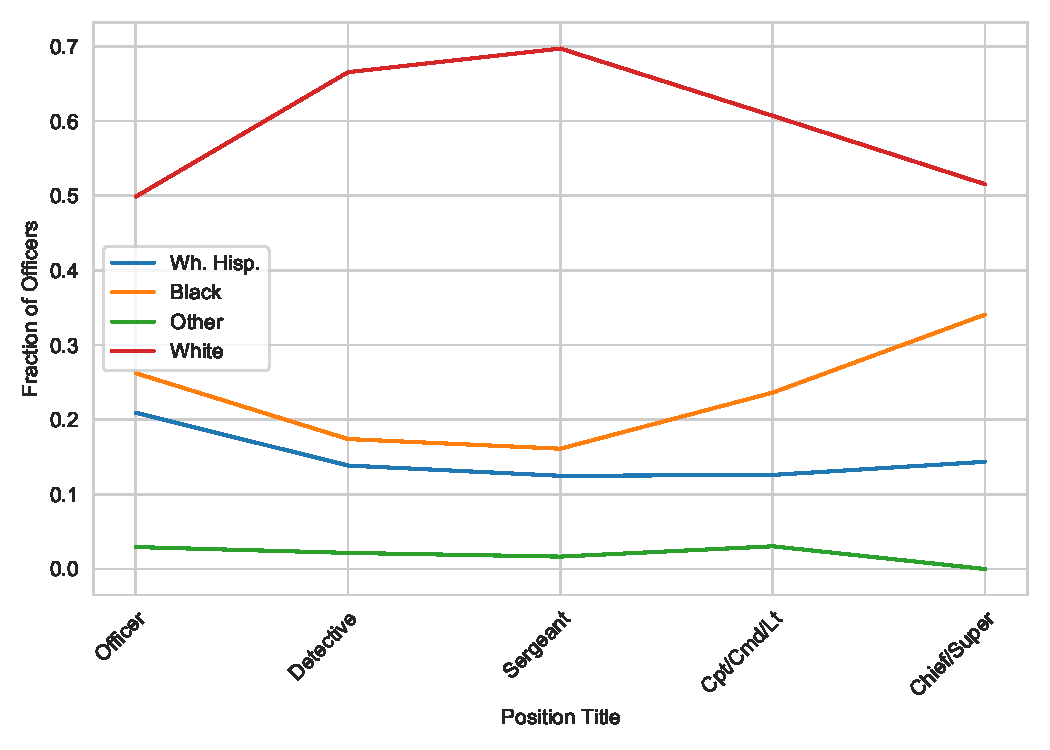
\includegraphics[width=\textwidth]{figs/position_race} 
\end{subfigure}
\begin{subfigure}{0.45\textwidth}
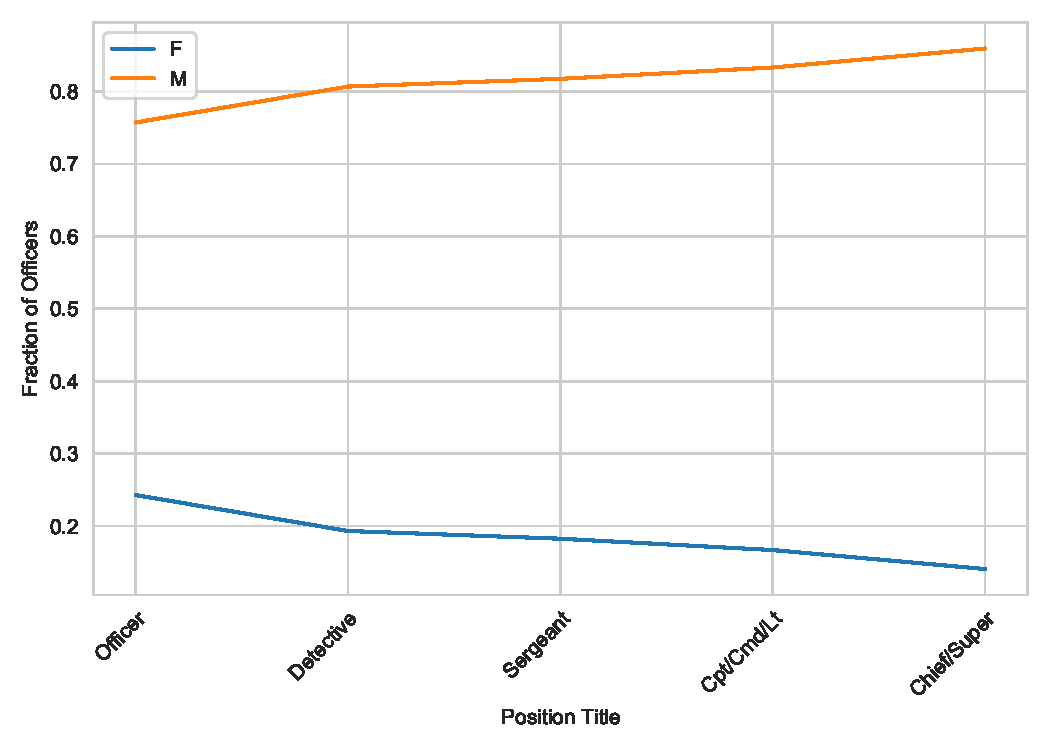
\includegraphics[width=\textwidth]{figs/position_gender} 
\end{subfigure}
\caption{Historical data from the CPD. Fraction of officers in representative positions 
per race category.} \label{fig:position}
\end{figure}



\begin{figure}[h] 
	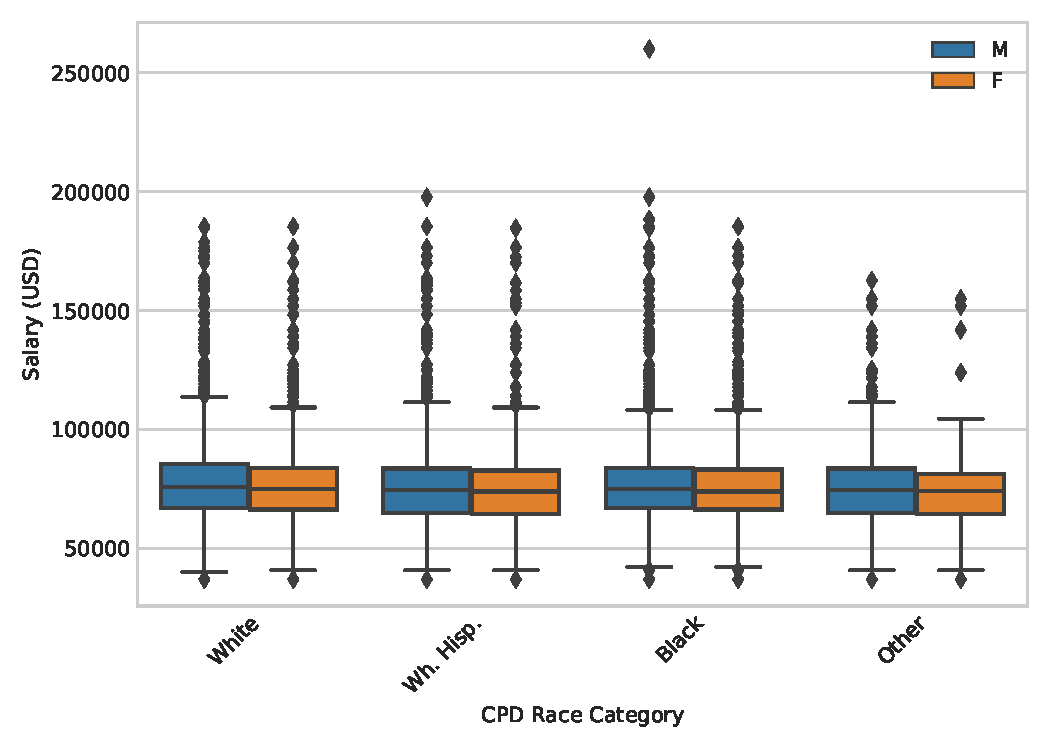
\includegraphics[width=\textwidth]{figs/salary_by_race_gender} 
	\caption{Temporal data for TRRs. Left: time during the day; mid-left: time during the week; mid-right: month; right: year.} \label{fig:salary_gender_race}
\end{figure}

\begin{figure}[h]
	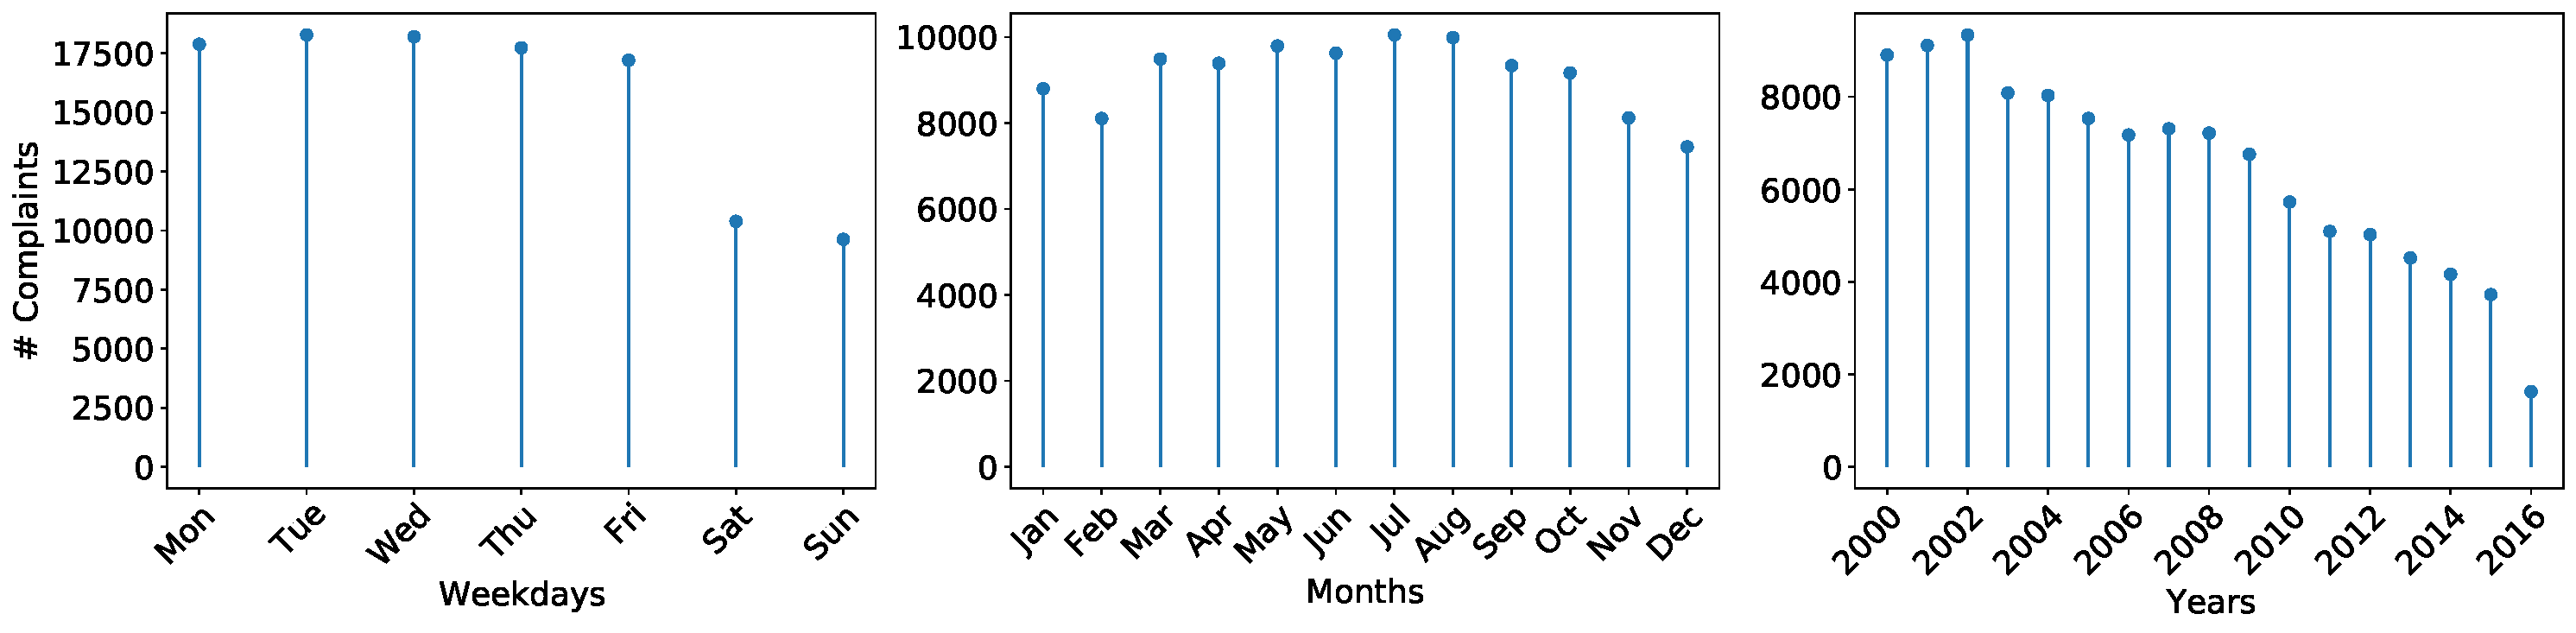
\includegraphics[width=\textwidth, clip, trim= 0 0 460 0]{figs/complaints_times} 
\caption{Complaints per day, month}
\end{figure}




\section{Breakdown of Missingness for Each Dataset}\label{sec:missingness}

\begin{table}[t!]
\caption{Missingness for the Roster data file}
\centering 
\begin{tabular}{lr}
\toprule
           Attribute &  \% Missing \\
\midrule
           last\_name &        0.0 \\
          first\_name &        0.0 \\
      middle\_initial &       17.9 \\
              gender &        0.0 \\
                race &        0.9 \\
           birthyear &        8.5 \\
                 age &        0.4 \\
              status &       10.3 \\
    appointment\_date &        0.6 \\
         position\_no &        1.6 \\
position\_description &       13.0 \\
             unit\_no &        4.0 \\
    unit\_description &       13.0 \\
    resignation\_date &       44.0 \\
               star1 &       21.7 \\
               star2 &       73.1 \\
               star3 &       90.8 \\
               star4 &       97.2 \\
               star5 &       99.3 \\
               star6 &       99.8 \\
               star7 &      100.0 \\
               star8 &      100.0 \\
               star9 &      100.0 \\
              star10 &      100.0 \\
              star11 &      100.0 \\
               sworn &       60.3 \\
             unit\_id &       60.3 \\
         unit\_detail &       91.6 \\
                star &       60.3 \\
                 uid &        0.0 \\
\bottomrule
\end{tabular}
\end{table}

\begin{table}[t!]
\caption{Missingness for the Unit Assignments data file}
\centering 
% Missing:
\begin{tabular}{lr}
\toprule
 Attribute &  \% Missing \\
\midrule
       uid &        0.0 \\
   unit\_no &        0.0 \\
start\_date &        0.0 \\
  end\_date &       27.6 \\
\bottomrule
\end{tabular}
\end{table}


\begin{table}[t!]
\caption{Missingness for the Complaints data file}
\centering 
% Missing:
\begin{tabular}{lr}
\toprule
        Attribute &  \% Missing \\
\midrule
     complaint\_no &        0.0 \\
             beat &        0.8 \\
    location\_code &        0.0 \\
        street\_no &       23.7 \\
      street\_name &       22.4 \\
           apt\_no &       99.0 \\
             city &       20.2 \\
incident\_datetime &        0.0 \\
   complaint\_date &        0.0 \\
      closed\_date &        1.8 \\
\bottomrule
\end{tabular}
\end{table}

\begin{table}[t!]
\caption{Missingness for the Tactical Response Reports data file}
\centering 
\begin{tabular}{lr}
\toprule
                   Attribute &  \% Missing \\
\midrule
                      trr\_id &        0.0 \\
                       rd\_no &        0.1 \\
              cr\_no\_obtained &       78.4 \\
               subject\_cb\_no &        8.9 \\
                    event\_no &        0.0 \\
                        beat &        0.0 \\
                       block &        0.0 \\
            street\_direction &        0.1 \\
                 street\_name &        0.0 \\
                    location &        0.0 \\
                        date &        0.0 \\
                        time &        0.1 \\
           indoor\_or\_outdoor &        1.3 \\
          lighting\_condition &        1.4 \\
           weather\_condition &        1.7 \\
                 notify\_oemc &       16.1 \\
        notify\_dist\_sergeant &       16.1 \\
           notify\_op\_command &       92.0 \\
              notify\_det\_div &       92.0 \\
number\_of\_weapons\_discharged &        0.0 \\
           party\_fired\_first &       46.8 \\
                 duty\_status &        0.0 \\
                     injured &        0.0 \\
           member\_in\_uniform &        0.0 \\
              subject\_gender &        0.1 \\
                subject\_race &        1.2 \\
                 subject\_age &        0.0 \\
           subject\_birthyear &        0.0 \\
               subject\_armed &        0.1 \\
             subject\_injured &        0.1 \\
      subject\_alleged\_injury &        0.1 \\
                         uid &        0.0 \\
\bottomrule
\end{tabular}
\end{table}


\begin{table}[t!]
\caption{Missingness for the Unit Names data file}
\centering 
\begin{tabular}{lr}
\toprule
       Attribute &  \% Missing \\
\midrule
         unit\_no &        0.0 \\
unit\_description &       10.6 \\
   active\_status &       12.3 \\
     status\_date &       12.3 \\
\bottomrule
\end{tabular}
\end{table}


\begin{table}[t!]
\caption{Missingness for the Awards data file}
\centering 
\begin{tabular}{lr}
\toprule
               Attribute &  \% Missing \\
\midrule
                     uid &        0.0 \\
                    star &       21.3 \\
             position\_no &        8.2 \\
    position\_description &        0.0 \\
      award\_request\_date &        0.0 \\
        award\_ref\_number &        0.0 \\
              award\_type &        0.0 \\
     requester\_last\_name &        0.7 \\
    requester\_first\_name &        0.7 \\
requester\_middle\_initial &       93.0 \\
             tracking\_no &       40.1 \\
          current\_status &        0.0 \\
     incident\_start\_date &        0.0 \\
       incident\_end\_date &       13.2 \\
    incident\_description &       91.8 \\
           ceremony\_date &       86.9 \\
\bottomrule
\end{tabular}
\end{table}

\begin{table}[t!]
\caption{Missingness for the Salary data file}
\centering 
\begin{tabular}{lr}
\toprule
              Attribute &  \% Missing \\
\midrule
                    uid &        0.0 \\
                   year &        0.0 \\
                 salary &        0.0 \\
   position\_description &        0.0 \\
              pay\_grade &        0.0 \\
present\_posn\_start\_date &       20.7 \\
           officer\_date &        0.6 \\
        employee\_status &        0.0 \\
\bottomrule
\end{tabular}
\end{table}


\end{document}
